%We moeten even beslissen welke van de twee we willen gebruiken
\documentclass[11pt]{uvamath}
%\documentclass[11pt]{amsart}
\usepackage{graphicx}
\usepackage[pdfborder={0 0 0}]{hyperref}

\usepackage{amssymb}
\usepackage{amsmath}
\usepackage{amsthm}

\usepackage{parcolumns}

\usepackage{caption}
\usepackage{subcaption}
\usepackage{geometry}
\usepackage{lipsum}

% PYTHON CODE
\usepackage{listings}
\usepackage{color}

\DeclareCaptionFont{black}{ \color{black} }
\DeclareCaptionFormat{listing}{
  \parbox{\textwidth}{\hfill#3}
}
\captionsetup[lstlisting]{ format=listing, textfont=black, singlelinecheck=false, margin=0pt, font={footnotesize} }

\definecolor{dkgreen}{rgb}{0,0.6,0}
\definecolor{gray}{rgb}{0.5,0.5,0.5}
\definecolor{mauve}{rgb}{0.58,0,0.82}

\lstset{
  language=Python,
  aboveskip=3mm,
  belowskip=3mm,
  frame=single,
  showstringspaces=false,
  columns=flexible,
  basicstyle={\small\ttfamily},
  numbers=none,
  numberstyle=\tiny\color{gray},
  keywordstyle=\color{blue},
  commentstyle=\color{dkgreen},
  stringstyle=\color{mauve},
  breaklines=true,
  breakatwhitespace=true,
  captionpos=b,
  tabsize=3
}
%PYTHON CODE

\usepackage[dutch]{babel}
\usepackage{a4wide}
\usepackage{algpseudocode}
\usepackage{algorithmicx}
\usepackage[square,super]{natbib}

\makeatletter
%replaces : \def\@endtheorem{\endtrivlist\@endpefalse }
% with:
%\def\@endtheorem{\endtrivlist}
\makeatother

\newcommand{\R}{\mathbb{R}}
\newcommand{\N}{\mathbb{N}}
\newcommand{\Z}{\mathbb{Z}}
\newcommand{\C}{\mathbb{C}}
\newcommand{\A}{\mathbb{A}}
\newcommand{\Q}{\mathbb{Q}}
\newcommand{\F}{\mathbb{F}}
\newcommand{\e}{\epsilon}
\renewcommand{\O}{\mathcal{O}}

\newcommand{\FFT}{\text{FFT}}

\theoremstyle{plain}                    
\newtheorem{stelling}{Stelling}[chapter]
\newtheorem{lemm}[stelling]{Lemma}     
\newtheorem*{algo}{Algoritme}      

\theoremstyle{definition}
\newtheorem{definitie}[stelling]{Definitie}  

\theoremstyle{remark}
\newtheorem{gevolg}{Gevolg}[stelling]
\newtheorem*{opmerk}{Opmerking}
\newtheorem*{voorbeeld}{Voorbeeld}

\newcommand{\eq}[1]{\begin{eqnarray*} #1 \end{eqnarray*}}
\newcommand{\mogelijkheden}[1]{\begin{cases} #1 \end{cases}}
\newcommand{\repr}[1]{{#1}^{\!\!-1}}

\newcommand{\coefficient}{co\"effici\"ent}
\newcommand{\coefficienten}{co\"effici\"enten}

\newcommand{\dx}{\text{d}x}
\newcommand{\dy}{\text{d}y}
\newcommand{\dz}{\text{d}z}
\newcommand{\largediv}{\,\big|\,}
\newcommand{\Ldnorm}[1]{{||#1||_{L_2}}}
\newcommand{\inpr}[2]{\langle #1 , #2 \rangle}
\newcommand{\DFT}{\text{DFT}}
\newcommand{\dpii}{{2\pi i}}
\newcommand{\abso}[1]{{\left| #1 \right|}}
\renewcommand{\d}[1]{{\mathrm{d} #1}}

\setlength\parindent{0pt}
\parskip = \baselineskip
\setcounter{tocdepth}{2}
\setcounter{secnumdepth}{1}

\title{JPEG-2000: de wondere wereld van Wavelets}
\date{\today}
\author[10219242, janner@gmail.com]{Jan Westerdiep}
\author[10191429, ovangarderen@gmail.com]{Ogier van Garderen}
\what{Projectverslag jaar 2}
\supervisors{Rob Stevenson}
%\secondgrader{dr.\ Ben Moonen}
\coverimage{
	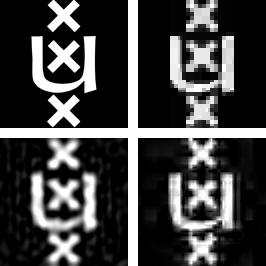
\includegraphics[width=0.6\linewidth]{plaatjes/voorkant.png}
}

\begin{document}
\maketitle

\begin{abstract}
\lipsum[2-3]

Op het voorblad is te zien, vanaf linksboven en dan met de klok mee:
\begin{itemize}
	\item Het originele UvA logo-plaatje;
	\item Compressie met een Haarwavelet waarbij 1\% van de data opgeslagen is;
	\item Compressie met een Daubechies-2 wavelet met 1\% van de data;
	\item Compressie met een Fouriertransformatie met 1\% van de data.
\end{itemize}
\end{abstract}

\tableofcontents
\newpage
\chapter{Intro}
\section{Signaaluitbreiding}
\label{signaal}
Beide algoritmes kunnen enkel omgaan met signalen die een tweemacht lang zijn. Om te zorgen dat een willekeurig signaal ook getransformeerd kan worden, moet het dus uitgebreid worden voorbij zijn definitiegebied. De meeste bronnen onderscheiden de volgende manieren om het signaal uit te breiden. Laat $x_1, x_2, \ldots x_n$ het signaal.
\begin{description}
\item[Zero-padding] $x' = 0, \ldots, 0| x_1, x_2, \ldots, x_n| 0, \ldots, 0$. Het gevolg van deze uitbreiding is dat het signaal niet langer continu hoeft te zijn op de randen;
\item[Constant padding] $x' = x_1, \ldots, x_1| x_1, x_2, \ldots, x_n| x_n, \ldots, x_n$. Het gevolg is nu dat het signaal geen continue afgeleide meer hoeft te hebben;
\item[Symmetric padding] $x' = x_n, \ldots, x_1| x_1, x_2, \ldots, x_n| x_n, \ldots, x_1$. Het gevolg is nu dat het signaal geen continue afgeleide meer hoeft te hebben;
\item[Periodic padding] $x' = x_1, \ldots, x_n| x_1, x_2, \ldots, x_n| x_1, \ldots, x_n$. Het nieuwe signaal hoeft wederom niet continu te worden.
\end{description}
Wij hebben ervoor gekozen om signalen uit te breiden door middel van zero-padding.

\chapter{Fourier}
\label{fourierH}

Bij het analyseren van periodieke functies is de Fouriertransformatie het gereedschap bij uitstek.
Het is een manier om een signaal te karakteriseren aan de hand van een bereik aan frequenties en dit maakt het een overtuigende manier om `nette' periodieke functies te beschrijven.
We kunnen de eis van periodiciteit ook loslaten als we naar functies op een interval kijken door dit op te vatten
als \'e\'en fase van een periodieke functie.

Iets concreter kijken we dus naar functies $f \in L_2([a,b])$. De basisfuncties waarmee we vervolgens de analyse uitvoeren worden gegeven door de complexe $e$-machten.
\begin{definitie}[Fourierbasis] Bekijk de functieruimte $L_2([a,b])$. We defini\"eren de verzameling $F_{a,b}$ 
door:
\[
  F_{a,b} := \left\{ \phi_k(x) = \tfrac{1}{\sqrt{b-a}} e^{\dpii \cdot k \frac{x-a}{b-a}} \largediv k \in \Z \right\}
\]
We noemen $F_{a,b}$ de Fourierbasis van $L_2([a,b])$.
\end{definitie}
Het woord basis is hier met recht gebruikt. Het is immers bekend dat de complexe $e$-machten loodrecht staan onder
het inproduct op $L_2$. 
Om nu een willekeurige functie te schrijven in deze basis, introduceren
we de Fouriergetransformeerde.
\begin{definitie}[Fouriertransformatie]
Zij gegeven een functie $f\in L_2([a,b])$. Schrijf dan $\hat f : \Z\to\C$ met entries gedefinieerd volgens:
\[
  \hat f [k] = \frac{1}{\sqrt{b-a}} \cdot \inpr{f}{\phi_k} = \frac{1}{b-a} \int_a^b f(x) \cdot e^{-2 \pi i \cdot k \frac{x-a}{b-a}}\d{x}.
\]
We noemen $\hat f$ de Fouriergetransformeerde van $f$.
\end{definitie}
\begin{definitie}[Inverse Fouriertransformatie]
  Gegeven een Fouriergetransformeerde $\hat f$ van een functie $f \in L_2([a,b])$, is de reconstructie $f^\circ$ van $f$ gegeven door:
  \[
    f^\circ (x) = \sum_{k=-\infty}^\infty \hat f [k] \phi_k(x).
  \]
\end{definitie}

In \cite{fourier-rec} is aangetoond dat $f^\circ$ een reconstructie geeft van $f$ die voldoet aan: 
\begin{eqnarray}
  \Ldnorm{f-f^\circ}{a,b}=0 \quad\quad \text{wanneer }& f\in L_2([a,b]) \\
  f(x) = f^\circ(x) \quad\quad \text{wanneer }& f \in C^1.
\end{eqnarray}
Merk op dat $\Ldnorm{f-f^\circ}{a,b}=0$ niet betekent dat $f - f^\circ = 0$.

%-----------------------------------------------------------------------------------------------------------------
\section{De \emph{Discrete Fourier Transform}}
Zoals we gezien hebben in het voorafgaande, kan de Fouriertransformatie gebruikt worden om continue signalen te karakteriseren door verschillende frequenties. 
Een groot gebied binnen de signaalanalyse is echter van discrete aard aangezien hier veelal digitale instrumenten worden gebruikt.

Om discrete signalen te analyseren lijkt het voor de hand te liggen om een deze als stapfuncties te zien;
een stapfunctie zit immers in $L_2$. De discontinu\"iteiten van de stapfunctie leiden echter tot ongewenste resultaten.
Elke reconstructie in termen van eindig veel continue basisfuncties is namelijk weer continu,
zodat voor een perfecte reconstructie van een stapfunctie met deze methode altijd een oneindige rij co\"effici\"enten nodig is. 
Bovendien is het moeilijk om uit deze co\"effici\"enten relevante informatie te destilleren over de aard van het signaal.

In plaats van de discrete signalen in te bedden in $L_2$ zullen we ze beschouwen als rijen in $\ell_2$ (zie sectie \ref{ruimtes}).
Hiervoor zullen we de Fourier-basis discretiseren en ons richten op de ruimte $\R^n$.
We veranderen daarvoor de co\"ordinaten naar een discrete $j$ volgens
\[
\frac{x-a}{b-a} \leftrightarrow \frac j n 
\]
Op deze manier zal de discretisatie in de limiet naar het continue geval overgaan. 

\begin{definitie}[Discrete Fourierbasis] Gegeven zij de ruimte $\C^n$. Defini\"er dan de verzameling
\[
  S_n := \left\{ s_k [j] = e^{\dpii\cdot k j/n } \largediv k,j \in \{1, \ldots, n\} \right\},
\]
als de \emph{discrete Fourierbasis} op deze ruimte met basisvectoren $s_k$.
\end{definitie}
We weten dat de basisvectoren loodrecht staan vanwege de eigenschap:
\[
  \inpr{s_k}{s_j} = 
  \sum_{m=1}^n s_k[m]\cdot \overline{s_j[m]} = 
  \sum_{m=1}^n e^{\dpii\cdot m (k-j)/n} =
  \begin{cases}
    0 \quad \text{als } k\neq j\\
    n \quad \text{als } k = j.
  \end{cases}
\]
Hierdoor kunnen we een discreet signaal $x$ schrijven in termen van $S_n$ 
een vector van inproducten te defini\"eren.
We noemen $X$ de discrete Fouriertransformatie (DFT) met entries:
\[
  X[k] = \tfrac{1}{n} \inpr{x}{s_k} \quad k\in\{1, \ldots ,n\}.
\]
Vervolgens hebben we een inverse voor deze operatie die $X$ afbeeldt op de reconstructie $x^\circ$ volgens:
\[
  x^\circ[j] = \inpr{X}{s_j^{-1}} \quad j\in \{1, \ldots, n\}.
\]
Waarbij we de notatie $s_j^{-1} = (s_j[1]^{-1},\ldots, s_j[n]^{-1})$ gebruiken.
Vanwege de orthogonaliteit van de basis $S_n$ is dit een perfecte reconstructie ($x[k] = x^\circ[k]$).

Om de claim te ondersteunen dat de DFT-methode een echte discretisatie is van de continue Fouriertransformatie,
willen we bewijzen dat deze algoritme voor een steeds fijnere selectie van waardes van een functie in de 
limiet hetzelfde resultaat geeft als de continue Fouriertransformatie. 
Zoals gebruikelijk bij het overschakelen van een discrete naar een continue setting kunnen we dit doen 
door de definitie van de Riemannintegraal toe te passen op de sommatie die voor handen ligt.

\begin{stelling}[Limiet van discrete Fouriertransformatie]
  Gegeven zij een functie $f\in L_2([a,b])$. Bekijk een discretisatie van $f$ in $n$ gelijke intervallen zodat de discrete $f$ precies 
  de randwaarde van elk interval inneemt.
  Dan geldt dat de discrete Fouriergetransformeerde limiteert naar de algemene Fouriergetransformeerde wanneer $n\to\infty$.
\end{stelling} 
\begin{proof}[Bewijs]
Gegeven een interval $[a,b]$ kunnen we een partitie $P$ maken in $n$ gelijke delen: laat $P=\{a=t_0,t_1,..,t_n=b\}$ met $t_j = a+\tfrac{j(b-a)}{n}$.
We discretiseren onze functie $f$ door uit elk interval $[t_{j-1},t_{j}]$ van de partitie de randwaarde in 
$x_j = t_j$ te selecteren, dus
\[
f[j] = f(x_j) = f(\frac{b-a}{n}j + a).
\]
De DFT van de discrete functie $f[\cdot]$ wordt dan gegeven door:
\[
F[k] = \frac1n\sum_{j=1}^n f[j] \cdot s_k^{-1}[j].
\]
We schrijven dit om in termen van onze non-discrete functie door $x_j\in[a,b]$ 
te vervangen door zijn discrete tegenhanger en krijgen zo:
\begin{eqnarray*}
  F[k] =& \frac{1}{n} \sum_{j=1}^n f[j]\cdot s_k^{-1}[n\cdot\tfrac{x_j-a}{b-a}] \\
       =& \frac{1}{n} \sum_{j=1}^n f(x_j)\cdot e^{-\dpii \cdot k \tfrac{x_j-a}{b-a}}\\
       =&  \frac{1}{\sqrt{b-a}}\sum_{j=1}^n f(x_j)\cdot \phi^*_k(x_j) \cdot\frac{b-a}{n} 
\end{eqnarray*}
We merken op dat de term $\frac{b-a}{n}$ precies de grootte is van de intervallen van de partitie 
en dat we het geheel omgeschreven hebben in termen van onze continue functies $f$ en $\phi_k$.
Omdat het product $f\cdot\phi_k$ integreerbaar is moet voor elke partitie $P$ met 
waarden in punten $x_j$ uit elk interval deze sommatie convergeren naar de integraal
\[
  \frac{1}{\sqrt{b-a}} \int_{[a,b]} f(x) \phi^*_k(x) \d{x}
\]
wanneer we de maaswijdte ($\tfrac{b-a}{n}$) naar $0$ laten gaan. \cite{shilov}
Dit is duidelijk het geval wanneer we de limiet $n\to\infty$ nemen. 
Dus is de DFT een goede discretisatie van de Fouriergetransformeerde. 
\end{proof}

%-----------------------------------------------------------------------------------------------------------------
\section{De Fast Fourier Transform}
\label{fft_sec}
De snelheid van de DFT-algoritme valt in de praktijk nogal tegen. Het nemen van $n$ inproducten over vectoren 
van lengte $n$ heeft namelijk een tijdscomplexiteit van $\O(n^2)$. Dit staat de directe implementatie van de DFT 
voor praktische toepassingen in de weg. Daarom is er een alternatieve algoritme, de \emph{Fast Fourier Transform}.

%%%%%
\begin{algo}[Fast Fourier Transform]
Gegeven een inputsignaal $x$ van lengte $n=2^m$, geeft het algoritme $\FFT$ 
een lijst terug van waardes $X$ van lengte $n=2^m$ als volgt:

Als $m=0$ dan geeft de $\FFT$ de lijst (van \'e\'en element) direct terug:
\[
X = x.
\]
Wanneer $m\neq0$ splitsen we de lijst $x$ op in lijsten $\e,o$ van zijn even en oneven indices:
\eq{
  \e[k]   =& x[2k]   &\quad \text{voor } k < n/2,\\
   o[k]   =& x[2k+1] &\quad \text{voor } k < n/2.
}
Vervolgens voeren we hierop het $\FFT$ algoritme uit om de volgende lijsten te verkrijgen:
\eq{
  E =& \FFT(\e), \\
  O =& \FFT(o).
}
Hiermee wordt de output van de algoritme geconstrueerd volgens:
\[
  X[k] = \left\{\begin{array}{llll}
    E[k]         &+& e^{-\dpii k/n}\cdot O[k] &  k< n/2, \\
    E[k-n/2] &-& e^{-\dpii (k-n/2)/n}\cdot O[k-n/2] &  k\geq n/2.
  \end{array}\right.
\]
\end{algo}
%%%%%

Dit is dus een recursief gedefinieerde algoritme dat een signaal meermaals halveert.
Het is gegarandeerd dat deze algoritme afloopt vanwege de conditie op $m=0$ samen met de halvering van de input bij elke stap. 
Een belangrijke voorwaarde voor de relevantie van de FFT is nu dat de algoritme hetzelfde resultaat geeft als de DFT-algoritme en dit zullen.
\begin{stelling}
  Het uitvoeren van de Fast Fourier Transform algoritme op een datasetgeeft
  dezelfde getransformeerde als de discrete Fouriertranformatie.
\end{stelling}
\begin{proof}[Bewijs]
We bewijzen met inductie naar $n$. Onze aanname is dat de FFT-algoritme voor $x$ van lengte $n=2^m$ gelijk is aan de DFT van $x$, ofwel
\eq{
  X[k] = \sum^{n}_{k=1} x[j] \cdot e^{-2\pi i \cdot jk/n}.
}
Dit geldt duidelijkerwijs wanneer $m=0$, onze basisstap. Hiervoor geldt namelijk:
\eq{
  X[k] = x[k] = x[1] = \sum^{2^0}_{k=1} x[j] \cdot e^{-2\pi i \cdot 1/2^0}.
}
Vervolgens passen we inductie toe naar $m$ door onze aanname voor $m-1$ te gebruiken. We vullen hier $E[k]$ en $O[k]$ in de vergelijking voor $X[k]$ in, deze hebben immers lengte $n=2^{m-1}$.
\eq{
  X[k] = \left\{\begin{array}{llll}
    \sum^{n/2}_{j=1} \e[j] 
    \cdot e^{-2\pi i \cdot kj \cdot 2/n} &+& 
    e^{-2\pi i \cdot k/n}
    \sum^{n/2}_{j=1} o[j] 
    \cdot e^{-2\pi i\cdot kj \cdot 2/n} &  k< n/2 \\
    \sum^{n/2}_{j=1} \e[j] 
    \cdot e^{-2\pi i\cdot (k-n/2) j\cdot 2/n} &-& 
    e^{-2\pi i\cdot (k-n/2)/n}
    \sum^{n/2}_{j=1} o[j] \cdot e^{-2\pi i\cdot (k-n/2)j\cdot 2/n} &  k\geq n/2 
  \end{array}\right.
}
Merk op dat we de $e$-machten in het tweede geval kunnen vereenvoudigen volgens
\eq{
  e^{-2\pi i\cdot (k-n/2)j \cdot 2/n} 
  = e^{-2\pi i\cdot kj\cdot 2/n} \quad,\quad e^{-2\pi i\cdot(k-n/2)/n} 
= -e^{-2\pi i\cdot k/n},
}
waardoor het gevalsonderscheid wegvalt, aangezien beide vergelijkingen nu identiek zijn.
Het resultaat is $X[k]$ als sommatie over de lijsten $\e$ en $o$. Vul de relatie voor $\e$ en $o$ met $x$ in en neem de factor voor de oneven indices mee in de sommatie om te krijgen
\eq{
  X[k] = \sum^{n/2}_{j=1} x[2j] \cdot e^{-2\pi i\cdot k (2j)/n} + 
    \sum^{n/2}_{j=1} x[2j+1] \cdot e^{-2\pi i\cdot k (2j+1)/n} 
    = \sum^n_{j=1} x[j] \cdot e^{-2\pi i\cdot k j/n}.
}
Dit bewijst dat de FFT hetzelfde resultaat levert als de DFT-algoritme. Het bewijs voor de gelijkheid van de iDFT en de inverse FFT is 
hetzelfde wanneer men de substitutie $-2\pi i \rightarrow 2\pi i$ uitvoert.
\end{proof}

\begin{opmerk}
We hebben hier telkens aangenomen -- en zullen deze aanname ook doorzetten -- 
dat de lengte van het ingangssignaal een macht van $2$ is. Dit is een belangrijke
eigenschap waar de variant van de FFT-algoritme dat hier gebruikt wordt, door werkt. Deze versie van FFT wordt
 \emph{Radix-2 Decimation In Time} van Cooley-Tukey genoemd. Algemenere vormen van deze algoritme
worden ook toegepast in geoptimaliseerde algoritmes maar om de implementatie te versimpelen 
is voor Radix-2 gekozen. Eventuele verschillen in afmetingen tussen een signaal en 
een 2-macht zijn opgelost met signaalextensie, zoals eerder beschreven.
\end{opmerk}

%-----------------------------------------------------------------------------------------------------------------
\subsection{Complexiteit van de Fast Fourier Transform}
We zullen de claim bewijzen dat de complexiteit van de FFT werkelijk beter lager is dan die van de DFT.
Hiervoor hebben we de volgende stelling uit de Complexiteitstheorie nodig.
\begin{stelling}[ Akra-Bazzi \cite{akra-bazzi}]
\label{akra}
    Zij $T:\N\to\R$ een recurrente betrekking van de vorm
    \[
    T(n) = \begin{cases}
      c_0 &\text{ als } n \leq d, \\
      a T(n/b) + f(n) &\text{ anders,} \\
    \end{cases}
    \]
    waarbij $a,b,d\in\N$, $c_0\in\R$ en $f$ een functie $f:\N\rightarrow\R$ die voldoet aan 
    \[
    \exists k \in \N \,:\, f(n) \in \theta(n^{\log a/\log b} \log^k n),
    \]
    dan wordt de orde van $T(n)$ gegeven door:
    \[
      T(n) \in \theta(n^{\log a / \log b} \log^{k+1}n).
    \]
\end{stelling}
De recurrente betrekking $T(n)$ kan gezien worden als het aantal stappen dat een machine nodig heeft om de algoritme uit te voeren.
Deze stelling is nu voldoende om een uitspraak te kunnen doen over de complexiteit.
\begin{stelling}[Complexiteit van de FFT]
  De Fast Fourier Transform algoritme heeft een tijdscomplexiteit van $\theta(n\log n)$ voor input van lengte $n=2^m$.
\end{stelling} 
\begin{proof}[Bewijs]
We schrijven de FFT in pseudocode.

\begin{algorithmic}
\Function{FFT}{$x$}
\State $n \gets \text{lengte}(x)$ \Comment Assumptie: $n = 2^m$ voor een $m$
\If {$n == 1$}
	\State{$X \gets x$}
\Else
	\State $E \gets FFT(x[0::2])$ \Comment{FFT op even indices}
	\State $O \gets FFT(x[1::2])$ \Comment{FFT oneven indices}
	\For{$i = 0$ to $n-1$}
		\If{$i < n/2$}
			\State $X[i] \gets E[i] + e^{-2i \pi k/n} \cdot O[i]$
		\Else
			\State $X[i] \gets E[i] - e^{-2i \pi k/n} \cdot O[i]$
		\EndIf
	\EndFor
\EndIf
\State \Return{$X$}
\EndFunction
\end{algorithmic}

Deze algoritme is recursief zodat we de complexiteit kunnen schrijven door middel van een recurrente betrekking. Laat hiervoor $T(n)$ het aantal berekeningen zijn dat de algoritme kost bij een invoersignaal van lengte $n$. We maken een gevalsonderscheid: als de lijst lengte $1$ heeft geven we deze direct terug (1 berekening). Bij een lijst van lengte groter dan $1$ splitsen we de lijst op in de even en oneven entries en voeren we op beiden weer FFT uit. Vervolgens voeren we nog $n$ maal een vast aantal (namelijk $N$) berekeningen uit om tot het eindresultaat te komen. In formulevorm geeft dit de \emph{recurrente betrekking}
\[
T(n) = \begin{cases}
    1 &\text{ als } n = 1 \\
    2\cdot T(n/2) + N\cdot n &\text{ anders}. \\
\end{cases}
\]

Gebruik nu stelling \ref{akra}. De recurrente betrekking voor de complexiteit van de FFT is inderdaad van dezelfde vorm als die van $T(n)$ in bovenstaande stelling.
Laat hiervoor namelijk $a=b=2$, $c_0=d=1$ en $f (n) = N\cdot n$, waarvoor geldt dat
\eq{
  f(n) \in \theta(n^{\log 2/\log 2} \log^0 n)=\theta(n).
}
Dit betekent dat $T(n) \in \theta(n \log n)$.
Hiermee hebben we bewezen dat de FFT en daarmee de iFFT binnen tijdscomplexiteit $\O(n\log n)$ lopen. 
\end{proof}

%-----------------------------------------------------------------------------------------------------------------
\section{Discrete Fourier Transform in meer dimensies}
Een eigenschap van de DFT-algoritme is dat het op een natuurlijke manier uit te breiden is naar hogere dimensies.
Per constructie is er dus een manier om de FFT ook te beschrijven voor hogere dimensies.
Het idee hierbij is om het Tensorproduct te nemen van meerdere bases.

\begin{definitie}[Multidimensionale Discrete Fourierbasis] 
Gegeven zij een signaalruimte van de vorm
$\R^{n_1} \times \R^{n_2} \times \ldots \times \R^{n_m}$.
We defini\"eren de multidimensionale discrete Fourierbasis behorende bij deze signaalruimte als
\[
  S_{\bold n}= S_{n_1}\otimes S_{n_2} \otimes \ldots \otimes S_{n_m} = 
  \left\{s_{\bold k}[{\bold j}]  = s_{k_1}[j_1]\cdot s_{k_2}[j_2]\cdot\ldots\cdot s_{k_m}[j_m] 
  \largediv s_{k_i} \in S_{n_i}, j_i \in \{1,\ldots, n_i\} \right\}
\]
Met basisvectoren $s_{\bold k}$, waar $\bold k$ een indexvector uit $\{1, \ldots, n_1\}\times\ldots\times\{1\ldots, n_m\}$ is.
Het feit dat dit een basis is, kan gevonden worden in \cite{topo}.
\end{definitie}

Wanneer we nu een $m$-dimensionaal signaal bekijken van lengte $n_1 \times \cdots \times n_m$, dan kunnen we
hierop een multidimensionale Fouriertransformatie op defini\"eren door het inproduct te generaliseren naar 
onze $m$-dimensionale signaalruimte.
\begin{equation}
  \label{algemeen_fourier_schema}
  X[\bold k] = \tfrac{1}{\bold n}
  \sum_{\bold j = \bold 1}^{\bold n} x[\boldsymbol j] s^{-1}_{\bold k}[\boldsymbol j] 
  =
  \left(\prod_{i=1}^m \tfrac{1}{n_i}\right) \cdot 
  \sum_{j_1=1}^{n_1} \ldots \sum_{j_m=1}^{n_m} 
  x[j_1,\ldots,j_m] \cdot 
  e^{-\dpii\cdot k_m \cdot j_m /n_m } \cdot \ldots \cdot e^{-\dpii\cdot k_1 \cdot j_1 /n_1 }.
\end{equation}

Echter, oals we voor de DFT al gezien hadden, is het uitrekenen van al deze inproducten erg tijdrovend.
We zullen daarom de Multidimentionale Discrete Fouriertransformatie (MDFT) op een andere manier defini\"eren 
zodat we beter gebruik kunnen maken van de DFT- en FFT-algoritmen die we al gevonden hebben.

\begin{algo}[Multidimensionaal DFT-algoritme]
Gegeven is een $m$-dimensionale input $x$ en een huidig level $t$. We schrijven de algoritme met output $X_t$ volgens
\begin{equation}
  \label{mdft_cases}
  X_{t}[\boldsymbol k] = \begin{cases}
  \DFT(X_{t-1}\largediv_{x_1 = k_1,\ldots,x_{t-1} = k_{t-1},x_{t+1} = k_{t+1},\ldots,x_m =k_m})[k_t] & \text{als } t>0,\\
  x[k_t] & \text{als } t=0.
  \end{cases}
\end{equation}

We beweren dat $X_m$ de multidimensionale Fouriertransformatie van een $m$-dimensionaal signaal geeft zoals
in \eqref{algemeen_fourier_schema}.
\end{algo}
\begin{proof}[Bewijs]
We voeren inductie naar de dimensie $m$. De inductiehypothese wordt dat voor een dimensie $m$ 
de vergelijking voor $X_m$ uit de algoritme gegeven wordt door \eqref{algemeen_fourier_schema}.

Als $m=1$ dan geldt:
\[
X_1[k_1] = DFT(X_0)[k_1] = DFT(x)[k_1],
\]
wat inderdaad de DFT in 1 dimensie geeft.


We gaan vervolgens door met de inductiestap. Laat $m > 1$. Schrijf kort
\[
\tilde X_{t-1}[k_t] := 
X_{t-1}\largediv_{x_1 = k_1,\ldots,x_{t-1} = k_{t-1},x_{t+1} = k_{t+1},\ldots,x_m =k_m}[k_t].
\]
Dan
\[
  X_m [\boldsymbol k] = 
  \DFT(\tilde X_{m-1})[k_m]
  = \frac 1 {n_m}\sum_{j_m=1}^{n_m} \tilde X_{m-1}[j_m] s^{-1}_{k_m}[j_m].
\]
We vatten $\tilde X$ op als een vector van lengte $n_m$ van $m-1$ dimensionale Fouriergetransformeerden.
Dit mag omdat
\[
X_{m-1}\largediv_{x_1=k_1,\ldots,x_{m-1}=k_{m-1}}[k_m] = X_{m-1}\largediv_{x_m=k_m}[k_1,\ldots,k_{m-1}]
\]
en daarmee is $X_{m-1}\largediv_{x_m=k_m}$ een $m-1$-dimensionaal object dat weer wordt gegeven door de relatie
in \eqref{mdft_cases}.

Omdat we de aanname voor $m-1$ dimensies al bewezen hebben geldt nu:
\[
X_m[\boldsymbol k]  = \frac 1 {n_m}\sum_{j_m=1}^{n_m} 
\left( \frac 1 {n_{m-1}} \sum_{j_{m-1}=1}^{n_{m-1}} \left ( \cdots 
\frac 1 {n_1} \sum_{j_1=1}^{n_1} 
x[j_1,\ldots,j_m] 
\cdot s^{-1}_{k_1}[j_1]
\cdots \right ) s^{-1}_{k_{m-1}}[j_{m-1}] \right) 
s^{-1}_{k_m}[j_m],
\]
wat precies is wat we wilden aantonen.
\end{proof}

Een belangrijk gevolg van de definitie van deze algoritme is dat de DFT-term in \eqref{mdft_cases}
gemakkelijk vervangen kan worden door een FFT-term. Beiden geven immers dezelfde output. 
Daarmee hebben we ook direct een MFFT gevonden.

\begin{opmerking}
Omdat bovenstaand algoritme niet in lineaire tijd loopt, neemt de wachttijd snel toe bij grote signalen en hogere dimensie. 
Dit wordt al snel een praktisch bezwaar en is dan ook een reden waarom we geen driedimensionale 
signalen hebben bekeken bij de implementatie van de Fouriertransformatie.
\end{opmerking}

%-----------------------------------------------------------------------------------------------------------------
\section{Compressie van een signaal onder FFT}
\label{daling_FFT}
Tot zover is de Discrete Fourieranalyse besproken met de gedachte van perfecte reconstructie,
aan de hand van een complete set co\"effici\"enten. Het doel van dit project is echter om
signalen te comprimeren: te reconstrueren aan de hand van een gelimiteerde dataset.
Om deze analyse te versimpelen, zullen in deze sectie een aantal inzichten aan bod komen die
de fout van zo'n reconstructie relateren aan de grootte van de dataset.

\iffalse
We zullen het convergentiegedrag gaan bepalen van de Fouriertransformatie voor functies die $C^k$ zijn.
We weten immers dat voor differentieerbare functies de Fourieranalyse perfect reconstrueerbaar is.
Met het convergentie gedrag van deze functies kunnen we dan kwantificeren hoe goed een functie te 
benaderen is met een eindige subset van de Fourier-getransformeerde.
We trachten daarom te bewijzen dat er een algebra\"isch verband bestaat tussen de fout en de frequentie
van de wavelets en bovendien een exponentieel verband tussen de fout en de `gladheid' van de functie.
\fi

\begin{lemm}[Riemann-Lebesque \cite{fourier-fout}]
\label{lebbie}
Wanneer $g \in L_1(\R)$, dan geldt 
\eq{
	G(z) = \left|\int_{-\infty}^\infty g(t) e^{- 2 \pi i z t} dt\right| \to 0 \text{ voor } z \to \infty.
}
\end{lemm}

\begin{stelling}[Daling van de co\"effici\"enten van de Fouriergetransformeerde]
\label{fourier_daling}
  Laat $f \in L_2([a,b])$. Stel er is een $n$ z\'o dat $f \in C^n$ en voor $0\leq j\leq n$ geldt dat $f^{(j)}(a) = f^{(j)}(b)$ -- $f$ en haar afgeleides zijn periodiek. Dan geldt dat de Fouriergetransformeerde $\hat f[k]$ in absolute waarde
  daalt met $k$ volgens $o(|k|^{-n})$.
\end{stelling}
\begin{proof}[Bewijs]
  Laat $f \in L_2([a,b])$ zodat $f$ voldoet aan de voorwaarden in de stelling voor een bepaalde $n$. 
  De Fouriergetransformeerde van $f$ wordt gegeven door:
  \eq{
    \hat f [k] = \tfrac{1}{\sqrt{b-a}} \inpr{f}{\phi_k}.
  }
  De constante in deze vergelijking heeft geen invloed op de orde, dus richten we ons op het inproduct. 
  We schrijven dit uit tot een integraal en voeren vervolgens -- $f$ is immers differentieerbaar -- parti\"ele
  integratie uit:
  \eq{
    \abso{\inpr{f}{\phi_k}} 
    =& \abso{\int_a^b f(x) e^{- 2 \pi i k \tfrac{x-a}{b-a}} dx}
    = \abso{\tfrac{b-a}{2 \pi i k}\left[ f(x) \cdot  e^{- 2 \pi i k \tfrac{x-a}{b-a}} \right]_a^b} 
    + \abso{\frac{b-a}{2 \pi i k}\right| \left|\int_0^1 f'(x) e^{-2 \pi i k \tfrac{x-a}{b-a}} dx} \\
    =& \abso{ f(b) \cdot 1 - f(a) \cdot 1} + \frac{b-a}{2 \pi \abso{k}} 
    \abso{ \int_a^b f'(x) e^{-2 \pi i k \tfrac{x-a}{b-a}} dx }
    = \tfrac{b-a}{2 \pi |k|} \left| \int_a^b f'(x) e^{-2 \pi i k \tfrac{x-a}{b-a}} dx \right|.
  }
  Hier hebben we gebruikt dat alle afgeleiden van $0$ tot $n$ periodiek zijn.
  Omdat $f$ van de klasse $C^n$ is en de afgeleiden weer periodiek zijn kunnen we dit herhaald toepassen en we verkrijgen daarmee
  \[
  \left| \int_a^b f(x) e^{-2 \pi i k \tfrac{x-a}{b-a}} dx \right| 
  = (\tfrac{2 \pi}{b-a} |k|)^{-n}\left| \int_a^b f^{(n)}(x) e^{- 2 \pi i k \tfrac{x-a}{b-a}} dx \right|.
  \]
  
  Vermenigvuldig beide kanten met $(\tfrac{2 \pi}{b-a} |k|)^n$ om te vinden dat
  \[
  (\tfrac{2 \pi}{b-a} |k|)^n \abso{\inpr{f}{\phi_k}} 
  = \abso{\int_a^b f^{(n)}(x) e^{- 2 \pi i k \tfrac{x-a}{b-a}} dx}.
  \]
  We willen graag lemma \ref{lebbie} toepassen op de rechterkant. 
  Merk daartoe op dat $f$ continu is op een gesloten interval, met als gevolg dat zij uniform continu is 
  en zij haar maximum en minimum hier dus aanneemt.

  Daarmee is de integraal van $|f|$ begrensd en dus is $f\in L_1([a,b])$. 
  Maar een functie die integreerbaar is op $[a,b]$ en daarbuiten nul, is integreerbaar op $\R$. 
  Dus we mogen Riemann-Lebesgue gebruiken om te zien dat
  \[
  (\tfrac{2 \pi}{b-a} |k|)^n \abso{\inpr{f}{\phi_k}} \to 0 \text{ als } |k| \to \infty.
  \]
  Maar dit betekent precies dat $\abso{\inpr{f}{\phi_k}} \in  o((\tfrac{2 \pi}{b-a} |k|)^{-n}) = o(|k|^{-n})$.
\end{proof}

De analyse van de co\"effici\"enten die we hier gegeven hebben vertaalt direct naar de fout die we krijgen
bij reconstructie van een Fouriergetransformeerde functie aan de hand van een kleinere set co\"effici\"enten.

\begin{gevolg}
Schrijf $f|_{N}$ voor de reconstructie met de eerste $N$ basisfuncties. Dan hebben we de relatie
\[
  || f - f|_N||^2_{L_2([a,b])} = \sum_{k=1}^\infty |\inpr{f-f|_N}{\phi_k}|^2 = \sum_{k=1}^\infty |\inpr{f}{\phi_k} 
  - \inpr{f|_N}{\phi_k}|^2 = \sum_{k=N+1}^\infty |\inpr{f}{\phi_k}|^2,
\]
vanwege de Parsevalgelijkheid \eqref{parseval}. Door stelling \ref{fourier_daling} zijn er $k_0$ en $c$ zodat $\abso{\inpr{f}{\phi_k}} < c\cdot k^{-n}$ voor $k > k_0$. Dus
\[
	\sum_{k=N+1}^\infty | \langle f, \phi_{k} \rangle |^2 \leq \sum_{k=N+1}^\infty c \cdot k^{-2n} < c \cdot \int_{N}^\infty x^{-2n} dx = c \cdot \left[ \frac{x^{1-2n}}{1-2n} \right]^\infty_N = c \cdot \frac{N^{1-2n}}{2n-1}.
\]
Dan
\[
N^{2(n-1)} \cdot \sum_{N+1}^\infty |\inpr{f}{\phi_k}|^2 < N^{2(n-1)} \cdot c \cdot \frac{N^{1-2n}}{2n-1} = \frac{c}{2n-1} N^{-1} \to 0 \quad \text{als } N\to\infty,
\]
wat precies betekent dat
 \[
\|f-f|_{N}\|^2_{L_2([a,b])} \in o\left ( N^{-2(n-1)} \right) 
\implies ||f - f|_{N}||_{L_2([a,b])} \in o\left(N^{-(n-1)}\right).
\]
\end{gevolg}

\subsection{De fout in het discrete geval}
Wanneer we een discrete functie bekijken zullen we het criterium van \emph{gladheid} niet kunnen gebruiken.
We beroepen ons daarom op de analogie tussen het discrete en non-discrete geval.

De gladheid van een discrete functie $f:A\to\R$ wordt bepaald door de verschillen \mbox{$f[x]-f[x+1]$},
wanneer de verschillen klein zijn en de verzameling $A$ groot is komt dit overeen met de afgeleide van een 
continue functie en zeggen we dat de functie glad is. Zo kunnen we analoga geven voor hogere afgeleiden.

We zullen in onze resultaten de discrete fout in kaart brengen door de zogenaamde PSNR-functie te gebruiken,
een logaritmische schaal die werkt over discrete signalen, welke ook als elementen uit $\ell_2$ kunnen worden beschouwd. Zie hiervoor hoofdstuk \ref{sectie_psnr}.



\chapter{Wavelets}
De Fouriertransformatie bestaat al honderden jaren en is een grote speler geworden in de \emph{signal processing}. Een groot nadeel van deze transformatie is dat zij slecht reageert op discontinue signalen door de globale dragers van de basisfuncties. Hierdoor worden alle Fourierco\"effici\"enten be\"invloed door een discontinu\"iteit.

In de loop van de vorige eeuw is een nieuwe transformatie ontstaan met een eigenschap die de Fouriertransformatie nooit kende. Deze noemt men nu ook wel de Wavelettransformatie.

\begin{definitie}
  Een wavelet is simpelweg een functie $\psi: \R \to \R$ die voldoet aan
  \[
  \int_{-\infty}^{\infty} \psi(t) dt = 0.
  \]
  Met deze functie $\psi$ kunnen we een familie functies $\psi_{u,s}$ bouwen door middel van schaling en translatie:
  \[
  \psi_{u,s}(t) := \frac{1}{\sqrt{s}} \psi\left(\frac{t-u}{s}\right).
  \]
\end{definitie}

Deze familie geeft aanleiding tot een Wavelettransformatie $W_f$ van $f$:
\[
W_f(u,s) = \int_{-\infty}^\infty f(t) \psi^*_{u,s}(t) dt.
\]

Het is nu mogelijk om wavelets te construeren die met deze schaling en translatie een basis voor de $L_2(\R)$ vormen. Over het algemeen kijken we dan naar
\[
\left\{ \psi_{j,n}(t) = \sqrt{2^j} \psi\left( 2^j t - n\right) : (j,n) \in \Z^2 \right\}.
\]
De kunst is nu om de basiselementen loodrecht op elkaar te laten staan, zodat er een orthogonale (en dus een orthonormale) basis gevormd wordt. Zie figuur~\ref{fig:wavelets} voor twee wavelets.

\begin{figure}[h]
  \centering
  \begin{subfigure}{0.48\linewidth}
    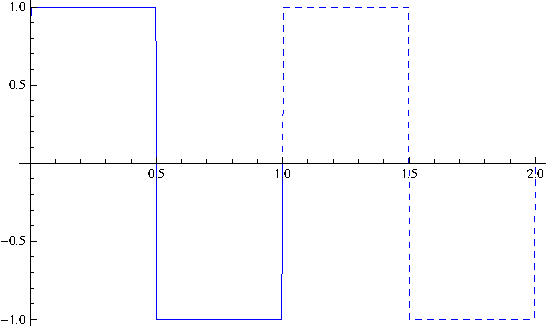
\includegraphics[width=\linewidth]{plaatjes/db1.pdf}
  \end{subfigure}
  \begin{subfigure}{0.48\linewidth}
    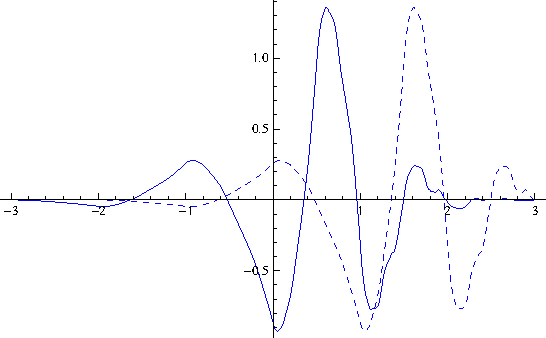
\includegraphics[width=\linewidth]{plaatjes/db4.pdf}
  \end{subfigure}
  \caption{Links: Haar. Rechts: De Daubechies-4. De gestippelde grafiek is een translatie naar rechts en staat in beide gevallen loodrecht op de continue lijn die de waveletfunctie voorstelt.}
\label{fig:wavelets}
\end{figure}

\begin{gevolg}We kunnen een functie $f$ in $L^2(\R)$ schrijven in deze basis:
  \[
  f(t) = \sum_{j=-\infty}^{\infty} \sum_{n=-\infty}^{\infty} \langle f, \psi_{j,n} \rangle \psi_{j,n}(t),
  \]
  waarbij $\langle \cdot, \cdot \rangle$ het standaardinproduct op de $L_2(\R)$ aangeeft.
\end{gevolg}

Het grote nadeel van de Fouriertransformatie maakt compressie van discrete signalen moeilijk. Veel van deze wavelets worden nu z\'o geconstrueerd dat dit probleem (deels) verholpen wordt. We zijn namelijk op zoek naar een wavelet die een eindige drager heeft. Het blijkt dat deze bestaat en dat er zelfs een hele grote verzameling wavelets is, elk met eigen gewilde eigenschappen.

Omdat wij naar de toepassing van wavelets binnen de beeldcompressie bekijken, zijn we natuurlijk vooral ge\"interesseerd in het discrete geval. We kijken dus naar de benadering van $f$. Dit geeft aanleiding tot een rij geneste ruimtes die uiteindelijk naar de $L_2(\R)$ toe gaat:

\begin{equation}
  \label{multires}
  V_0 \subset V_1 \subset \ldots \subset L_2(\R)
\end{equation}
genaamd een multiresolutie.
\begin{definitie}
  Een rij geneste ruimtes $\{ V_j: j \in \N_0 \}$ zoals in~\ref{multires} heet een multiresolutie wanneer voldaan wordt aan de volgende eigenschappen:
  \begin{eqnarray}
    \forall j, k: f(t) \in V_j \implies f(t - 2^j k) \in V_j, \\
    \forall j: V_{j-1} \subset V_j, \\
    \forall j: f(t) \in V_j \iff f(t/2) \in V_{j-1}, \\
    \bigcup_{j=0}^{\infty} V_j = \lim_{j\to\infty} V_j = L_2(\R), \\
    \text{ Er is $\phi: \R \to \R$ zo dat $\{ \phi(t-n): n \in \Z \}$ een orthonormale basis voor $V_0$ is.}
  \end{eqnarray}
\end{definitie}

\begin{voorbeeld} We bekijken een multiresolutie van stuksgewijs constante functies. De ruimte $V_j$ wordt hiermee
  \[
  V_j = \left\{ g(t) \in L_2(\R): g(t)\text{ is constant voor }t \in [n 2^{-j}, (n+1)2^{-j}) \right \}
    \]
    met $n \in \Z$. De basisfunctie $\phi$ voor $V_0$ wordt in dit geval $\phi(t) = 1_{[0,1)}(t)$.
\end{voorbeeld}

\section{Schalingsfuncties}
Gegeven zo'n orthonormale basis voor $V_0$ willen we graag een orthonormale basis voor $V_j$ construeren.
\begin{stelling}[{\cite[T7.1]{mallat}}]
  Laat $\{ V_j \}$ een multiresolutie en laat $\{\phi(t-n) \}$ de basis voor $V_0$. Laat verder
  \[
  \phi_{j,n}(t) := \sqrt{2^j} \phi\left( t2^j - n \right).
  \]
  Dan is $\{ \phi_{j,n}: n \in \Z \}$ een orthonormale basis voor $V_j$. De functie $\phi$ is ook wel de \emph{schalingsfunctie}.
\end{stelling}
\subsection{Benadering} De orthogonale projectie van $f$ op $V_j$ is, zoals we weten, de beste benadering van $f$ in $V_j$. Deze is nu te vinden door
\[
P_{V_j} f = \sum_{n=-\infty}^\infty \langle f, \phi_{j,n} \rangle \phi_{j,n}.
\]
De co\"effici\"enten $a_j[n] = \langle f, \phi_{j,n} \rangle$ geven ons op deze manier een discrete benadering van $f$ op resolutie $2^j$.

\section{Filters}
Wanneer we een schalingsfunctie $\phi$ defini\"eren (en dus een $V_0$), dan lijkt $V_1$ (en dus $V_j$) al redelijk beschreven te worden.\footnote{In stelling \ref{filter} wordt bewezen dat deze hele multiresolutie vast ligt.} We zullen daarom deze schalingsfunctie nader onderzoeken.

Per definitie van de multiresolutie weten we dat $V_{j-1} \subset V_j$. In het bijzonder geldt dat $\phi(t) \in V_0 \subset V_1$ en omdat $\{ \sqrt{2}\phi(2t - n): n \in \Z\}$ een orthonormale basis voor $V_1$ is, kunnen we $\phi(t)$ nu schrijven als
\[
\phi(t) = \sum_{n=-\infty}^{\infty} \left\langle \sqrt{2} \phi\left(2t-n\right), \phi(t) \right\rangle \sqrt{2}\phi(2t-n).
\]

\begin{definitie}
  Deze inproducten hebben een speciale naam, want de rij $\{h[n]: n \in \Z\}$ met
  \[
  h[n] := \left\langle \sqrt{2} \phi\left(2t-n\right), \phi(t) \right\rangle
  \]
  wordt nu ook wel de \emph{filter} van $\phi$ genoemd.
\end{definitie}
\begin{stelling}[{\cite[T7.2]{mallat}}]
  \label{filter}
  Laat $\phi \in L^2(\R)$ een schalingsfunctie die ook integreerbaar is. Dan ligt de multiresolutie vast.

  Andersom, als $h[n]$ een filter is zodat $\hat{h}(\omega)$ periodiek $2\pi$ is en continu differentieerbaar in een omgeving van $\omega = 0$ en als daarnaast geldt
  \begin{align*}
    \forall \omega \in \R: | \hat{h}(\omega)|^2 + |\hat{h}(\omega + \pi)|^2 = 2, \\
    \hat{h}(0) = \sqrt{2}, \\
    \inf_{\omega \in [-\pi/2, \pi,2]} |\hat{h}(\omega)| > 0,
  \end{align*}
  dan is de functie $\phi$ waarvan de Fouriergetransformeerde voldoet aan
  \[
  \hat{\phi}(\omega) = \prod_{p=1}^\infty \frac{\hat{h}(2^{-p}\omega)}{\sqrt{2}}
  \]
  een schalingsfunctie in $L^2(\R)$.
\end{stelling}
We zullen enkel de gevolgen gebruiken: namelijk dat de multiresolutie vast ligt met een goede keuze van $\phi$, en dat voor een goed gekozen $h[n]$, $\phi$ ook vast ligt.

\begin{voorbeeld}
  Bekijk weer het geval $\phi(t) = 1_{[0,1)}(t)$. Dan vinden we dat
    \[
    h[n] = \left\langle \sqrt{2} \phi\left(2t-n\right), \phi(t) \right\rangle = \begin{cases} \frac{1}{\sqrt{2}} & \text{ als } n \in \{0,1\} \\ 0 & \text{ anders.} \end{cases}
    \]
\end{voorbeeld}

\section{Terugkeer van de wavelet}
We weten dat $V_{j-1}$ bevat is in $V_{j}$. Laat nu $W_{j-1}$ het orthogonale complement van $V_{j-1}$ in $V_{j}$:
\begin{equation}
  \label{ruimterec}
  V_{j} = W_{j-1} \oplus V_{j-1}
\end{equation}
De projectie van $f$ op $V_{j-1}$ kan dus geschreven worden als som van projecties:
\begin{equation}
  \label{projectie_rec}
  P_{V_{j}} f = P_{V_{j-1}} f + P_{W_{j-1}} f.
\end{equation}
Omdat $V_j \subset V_{j+1}$ is alle informatie over $f$ die beschikbaar is in $V_j$, ook beschikbaar in $V_{j+1}$. Ook is het goed mogelijk dat door deze grovere benadering, informatie zoek gaat. Deze `details' worden op die manier zichtbaar in $P_{W_j} f$.

Het kan bewezen worden \cite[T7.3]{mallat} dat, gegeven een schalingsfunctie $\phi$ (en daarmee een filter $h$) er een functie $\psi$ bestaat zo dat
\[
\left\{ \psi_{j,n}(t) := \sqrt{2^j} \psi\left(2^jt - n\right) : n \in \Z \right\}
\] een orthonormale basis is voor $W_j$ en $\{ \psi_{j,n}: (j,n) \in \Z^2 \}$ een basis voor $L_2(\R)$. Deze functie is dan een \emph{orthogonale} wavelet, omdat $W_j \perp V_j$.
Omdat nu $W_j \subset V_{j+1}$ en dus in het bijzonder $\psi(t) \in W_0 \subset V_1$ en omdat $\{ \sqrt{2}\phi(2t-n): n \in \Z \}$ een orthonormale basis is voor $V_1$, kunnen we ook $\psi(t)$ in termen schrijven als:
\[
\psi\left(t\right) = \sum_{n=-\infty}^{\infty} \left\langle \psi\left(t\right), \sqrt{2}\phi(2t-n) \right\rangle \sqrt{2}\phi(2t-n).
\]
Ook deze inproducten hebben een speciale naam: de rij $g[n]$ met
\[
g[n] := \left\langle \psi\left(t\right), \sqrt{2}\phi(2t-n) \right\rangle
\]
wordt nu ook wel de filter van $\psi$ genoemd. De twee filters zijn gerelateerd aan elkaar volgens de vergelijking\cite[V13]{wavelet_filter}\cite[P958]{daubechies}
\begin{equation}
\label{highpassfilter}
g[n] = (-1)^{n}h[1-n].
\end{equation}

Zoals nu wel duidelijk geworden is, wordt met een filter $h$ (die voldoet aan bepaalde eigenschappen: zie stelling~\ref{filter}) een schalingsfunctie $\phi$ en een filter $g$ met waveletfunctie $\psi$ geconstrueerd.

\begin{voorbeeld}
  We keren nog een laatste keer terug naar het voorbeeld waarin $\phi(t) = 1_{[0,1)}$. We vinden met de gelijkheden uit voorgaande paragrafen dat
    \[
    \psi\left(t\right) = \sum_{n=-\infty}^{\infty} (-1)^{n}h[1-n] \sqrt{2}\phi(2t-n),
    \]
    en omdat $h[0] = h[1] = 2^{-1/2}, h[n] = 0$ voor $n \in \Z \setminus \{0,1\}$ zoals we eerder vonden, herschrijft dit tot
    \[
    \psi\left(t\right) = \sqrt{2}\left(\phi(2t) - \phi(2t - 1)\right)
    \]
    met als gevolg dat
    \[
    \psi(t) = \begin{cases} 1 & \text{ als } t \in [0,1/2) \\ -1 & \text{ als } t \in [1/2,1) \\ 0 & \text{ anders.} \end{cases}
    \]

    Deze wavelet $\psi$ wordt ook wel de Haarwavelet genoemd en is uitgevonden voor Alfred Haar in 1909, hoewel het onderzoeksgebied van de wavelets toen nog niet bestond. In het vervolg zullen we nog verdere aandacht aan deze wavelet besteden.
\end{voorbeeld}

\section{Het kiezen van een wavelet}
Bij het kiezen of vinden van een wavelet is men over het algemeen op zoek naar bepaalde eigenschappen. Voor compressie zijn we op zoek naar een wavelet die een klein aantal grote co\"effici\"enten en een groot aantal kleine teweeg brengt: een soort concentratie van de belangrijke informatie. Dit wordt vooral bepaald door drie factoren: gladheid van $f$ (waar we niks aan kunnen doen), de grootte van de drager (welke hierna aan bod komt) en de zogenaamde orde van de wavelet.

\begin{definitie}
  Wanneer de waveletfunctie loodrecht staat ($\langle \psi, q\rangle = 0$) op alle polynomen van graad $p-1$ of lager, spreken we van een wavelet van orde $p$. Dit komt overeen met te zeggen dat
  \[
  \int_{-\infty}^\infty x^k \psi(x) dx = 0 \text{ voor } k \in \{ 0, \ldots p-1 \}.
  \]
\end{definitie}

\begin{gevolg}
  Gevolg van deze eigenschap is dat we van de functie $f$ elk polynoom van graad $p-1$ af mogen trekken zonder een verschil in inproduct:
  \[
  \langle f, \psi_{j,n} \rangle = \langle f - q, \psi_{j,n} \rangle \text{ voor $q$ een polynoom van graad $p-1$}.
  \]
  Intu\"itief is deze eigenschap natuurlijk gewild: we winnen immers een heel stel keuzevrijheden. We zullen dit argument in een volgende sectie formaliseren.
\end{gevolg}

Eerder spraken we het verlangen uit om een wavelet met eindige drager te vinden zodat discontinu\"iteiten alleen lokaal zichtbaar zijn. We zullen hier de dragers van $h[n], \psi$ en $\phi$ aan elkaar relateren.

\subsection{Compacte drager}
Hoewel $\phi$ een functie uit $L_2$ is, en $h$ een functie uit $\ell_2$, is het toch mogelijk het begrip drager in beide ruimtes te beschrijven alsof ze hetzelfde zijn. Laat daartoe $h'$ de stuksgewijs constante functie van $\R$ naar $\R$ die $x$ stuurt naar $h(\lfloor x \rfloor)$. Dan is de drager van $h$ gedefini\"eerd als de drager van $h'$.

\begin{stelling}[{\cite[P7.2]{mallat}}]
  De volgende relaties gelden voor de dragers.
  \begin{enumerate}
  \item De schalingsfunctie $\phi$ heeft een compacte drager dan en slechts dan als het filter $h[n]$ een compacte drager heeft, en deze zijn hetzelfde.
  \item Als de drager van $\phi$ gelijk is aan $[N_1,N_2]$ dan is de drager van $\psi$ gelijk aan $[(N_1 - N_2 + 1)/2, (N_2 - N_1 + 1)/2]$.
  \end{enumerate}
\end{stelling}
\begin{proof}[Bewijs 1] Als $\phi$ een compacte drager heeft dan $h[n]$ ook: we weten dat
  \[
  h[n] = \left\langle \sqrt{2} \phi\left(2t-n\right), \phi(t) \right\rangle,
  \]
  dus er kunnen maar eindig veel $n$ ongelijk nul zijn. De omgekeerde bewering staat bewezen in \cite[P965-967]{daubechies}. TODO?

  Om deze dragers gelijk te krijgen, stel dat de drager van $h[n]$ gelijk $[N_1,N_2]$ is, en die van $\phi$ $[K_1, K_2]$. De drager van $\phi(t/2)$ is $[2K_1, 2K_2]$ en de drager van de rechterzijde van $\ref{phi_t2}$ is $[N_1 + K_1, N_2 + K_2]$. We concluderen dat $K_1 = N_1$ en $K_2 = N_2$.
\end{proof}
\begin{proof}[Bewijs 2]
  Kijk nu naar
  \[
  \psi\left(t\right) = \sum_{n=-\infty}^{\infty} g[n] \phi(2t-n) = \sum_{n=-\infty}^{\infty} (-1)^{n}h[1-n] \phi(2t-n).
  \]
  Met de informatie uit het begin van de stelling kunnen we de drager van de rechterkant vinden: $[N_1 - N_2 + 1, N_2 - N_1 + 1]$. De functie $\psi(t/2)$ is nu precies een dilatie met factor twee dus de drager van $\psi(t)$ moet wel gelijk zijn aan $[(N_1 - N_2 + 1)/2, (N_2 - N_1 + 1)/2]$.
\end{proof}

\subsection{Daubechieswavelets}
Hoewel de constructie van de Daubechieswavelet buiten het spectrum van dit artikel valt,\footnote{Voor een goede beschrijving van deze constructie, zie \cite{mallat} of \cite{daubechies}.} willen we toch een kort licht schijnen op deze speciale familie van wavelets. Deze worden gemaakt met de noties van eerder, namelijk dat we de drager willen minimaliseren maar de orde maximaliseren. Daubechies heeft bewezen\cite{daubechies} dat een filter $h$ met orde $p$, minimaal een drager van lengte $2p$ moet hebben. De zogenaamde Daubechieswavelet van orde $p$ heeft precies een filter van lengte $2p$. In het bijzonder is de Haarwavelet de eerste in de familie van Daubechieswavelets.

Wij hebben in het praktische deel van ons project aandacht besteed aan de zogenaamde Daubechies-2 wavelet die haar naam ontleent aan het feit dat zij van orde 2 is.

\begin{figure}[h]
  \centering
  \begin{subfigure}{0.48\linewidth}
    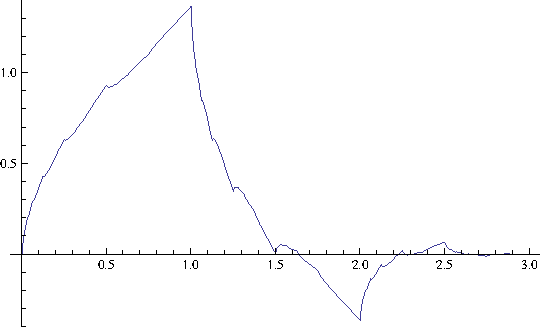
\includegraphics[width=\linewidth]{plaatjes/db2_phi.pdf}
  \end{subfigure}
  \begin{subfigure}{0.48\linewidth}
    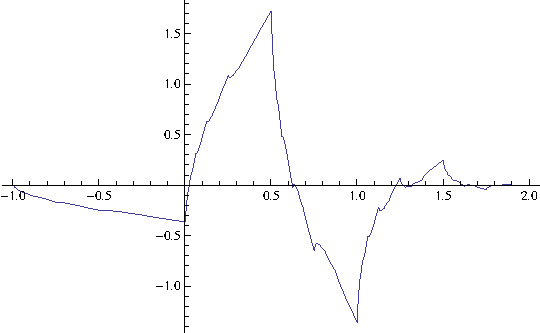
\includegraphics[width=\linewidth]{plaatjes/db2_psi.pdf}
  \end{subfigure}
  \caption{Links: de Daubechies-2 schalingsfunctie. Rechts: de Daubechies-2 waveletfunctie.}
\end{figure}

\section{Fast Wavelet Transform}

Door de recursieve relatie van de ruimtes in \ref{ruimterec} herhaald toe te passen,
kunnen we de ruimte $V_j$ schrijven in termen van $V_0$ en een scala aan
orthogonaal-complementsruimtes $W_k$.
\begin{equation}
  \label{ruimte_splitsing}
  V_j = V_k \oplus W_k \oplus \cdots \oplus W_{j-1} = \ldots
  = V_0 \oplus W_0 \oplus \cdots \oplus W_{j-1}
\end{equation}
We willen nu een functie $f$ benaderen in de ruimte $V_j$ door $P_{V_j}f$ te schrijven in
de basis van de ruimtes $V_0$ en de verschillende $W_k$. Hiervoor dienen we de inproducten
te bereken van $f$ met de basisvectoren in deze ruimtes.
We onderscheiden dan de \emph{approximatie}
co\"efficienten $a_j[n]$ en de \emph{detail} co\"efficienten $d_j[n]$, die
$f$ geven als projectie op  respectievelijk $V_j$ en $W_j$.

Het is echter veel rekenwerk om al deze co\"efficienten uit te rekenen, dit gebeurt immers
door het berekenen van integralen. We beperken ons daarom tot her uit rekenen van de
co\"efficienten op het niveau $j$ en proberen vervolgens een recursieve relatie te vinden
om hieruit de approximatie en detailco\"efficienten te vinden.

Vanwege de relatie in \ref{ruimterec} kunnen we de basisfuncties uit de ruimtes $W_{j-1}$,
$V_{j-1}$ schrijven in termen van de basisfuncties van de ruimte $V_j$.
We schrijven daarvoor $\phi_{j-1,n}$ om in termen van de basisfuncties $\phi_{j,k}$; evenzo
voor $\psi_{j-1,n}$.
\begin{equation}
  \label{phi_rec}
  \phi_{j-1,n} = \sum_{k=-\infty}^{\infty} \inpr{\phi_{j-1,n}}{\phi_{j,k}} \phi_{j,k}
\end{equation}
\begin{equation}
  \label{psi_rec}
  \psi_{j-1,n} = \sum_{k=-\infty}^{\infty} \inpr{\psi_{j-1,n}}{\phi_{j,k}} \phi_{j,k}
\end{equation}
We rekenen vervolgens de inproducten uit om deze om te schrijven naar een filterco\"efficient,
bekijk
\eq{
  \inpr{\phi_{j-1,n}}{\phi_{j,k}}
  =& \int_{-\infty}^\infty \sqrt{2^{j-1}}\phi(2^{j-1}t -n)
  \sqrt{2^{j}}\phi^\star(2^j t - k) \d{t}\\
  =& \int_{-\infty}^\infty \tfrac{1}{2^j} 2^{j-1}
  \sqrt{2} \phi(t') \phi(2t' - k + 2n) \d{t'}\\
  =& \inpr{\phi(t)}{\sqrt{2}\phi(2t-k+2n)} \\
  =& h[k-2n],
}
\eq{
  \inpr{\psi_{j-1,n}}{\phi_{j,k}}
  =& \int_{-\infty}^\infty \sqrt{2^{j-1}}\psi(2^{j-1}t -n)
  \sqrt{2^{j}}\phi^\star(2^j t - k) \d{t}\\
  =& \int_{-\infty}^\infty \tfrac{1}{2^j} 2^{j-1}
  \sqrt{2} \psi(t') \phi(2t' - k + 2n) \d{t'}\\
  =& \inpr{\psi(t)}{\sqrt{2}\phi(2t-k+2n)} \\
  =& g[k-2n],
}
waarbij we de co\"ordinaat-transformatie $t' = 2^{j-1}t - n$ hebben gebruikt.
Door nu aan beide zijden van vergelijkingen \ref{phi_rec}, \ref{psi_rec} het
inproduct met $f$ te nemen kunnen we de coe\"fficienten van de resolutie $2^{j-1}$ schrijven
in termen van de coe\"fficienten op de resolutie $2^j$.
\begin{equation}
  \label{approx_rec}
  a_{j-1}[n] = \inpr{f}{\phi_{j-1,n}}
  = \sum_{k=-\infty}^{\infty} h[k-2n] \inpr{f}{\phi_{j,k}}
  = \sum_{k=-\infty}^\infty h[k-2n] a_{j}[k]
  = (a_j \star \bar h)[2n]
\end{equation}
\begin{equation}
  \label{detail_rec}
  d_{j-1}[n] = \inpr{f}{\psi_{j-1,n}}
  = \sum_{k=-\infty}^{\infty} g[k-2n] \inpr{f}{\phi_{j,k}}
  = \sum_{k=-\infty}^\infty g[k-2n] a_{j}[k]
  = (a_j \star \bar g)[2n]
\end{equation}
Waarbij $\bar f: x \mapsto f(-x)$ en $x\star y$ de discrete convolutie aangeeft,
als kortere schrijfwijze van deze sommatie.
De relatie die hier gevonden is geeft aanleiding tot een algoritme.

\begin{algo}[Fast Wavelet Transform]
  Gegeven een rij co\"effici\"enten $a_j\in\R^{2^j}$ dan definie\"eren we een recursief
  algoritme $\mathrm{FWT}:\R^{2^j}\to\R^{2^j}$ volgens:\\
  Als $j=0$ dan geldt
  \[
  \mathrm{FWT}(a_j)[n] = a_j[n]
  \]
  Als $j>0$ bereken $a_{j-1}$ en $d_{j-1}$ volgens \ref{approx_rec}, \ref{detail_rec}.
  Vervolgens geldt
  \begin{equation}
    \label{FWT_cases}
    \mathrm{FWT}(a_j)[n] = \begin{cases}
      \mathrm{FWT}(a_{j-1})[n] & \text{als } n\leq 2^{j-1} \\
      d_{j-1}[n] & \text{als } n>2^{j-1} \end{cases}
  \end{equation}
\end{algo}
We gaan hierbij uit van een eindige filter en beschouwen onze ruimte $V_j$ als functies
op een interval in $\R$, dan versimpelen de oneindige sommaties in \ref{approx_rec},
\ref{detail_rec}. Voor een discrete functie $f\in\R^{2^j}$ kunnen we nu
$\mathrm{FWT}(f)$ nemen als de fast wavelet transform,
we nemen dan aan dat $\inpr{f}{a_{j,k}} = f[k]$ voor het
grootste niveau $V_j$. Deze aannames komen ruwweg neer op de bewering dat
$V_0 = \{\phi_{0,0}\}$ en dat zowel $\phi$ als $\psi$ een compacte drager heeft.

We kunnen vervolgens de transformatie inverteren aan de hand van het volgende algoritme
\begin{algo}[Inverse Fast Wavelet Transform]
  Gegeven een rij co\"effici\"enten $x_j\in\R^{2^j}$ dan definie\"eren we een recursief
  algoritme $\mathrm{iFWT}:\R^{2^j}\to\R^{2^j}$ volgens:\\
  Als $j=0$ dan geldt
  \[
  \mathrm{iFWT}(x_j)[n] = x_j[n]
  \]
  Als $j>0$ laat $x_{j-1}[n] = x_j[n]$ en $d_{j-1}[n] = x_j[n+2^{j-1}]$ voor
  $1\leq n\leq 2^{j-1}$. Bereken hiermee $a_{j-1} = iFWT(x_{j-1})$,
  dan geldt
  \begin{equation}
    \label{reconstr_FWT}
    \mathrm{iFWT}(x_j)[n] = (\breve a_{j-1}\star h)[n] + (\breve d_{j-1}\star g)[n]
  \end{equation}
  Waarbij $\breve y [2n] = y[n]$ en $\breve y [2n+1] = 0$.
\end{algo}
\begin{stelling}
  De iFWT (links) samengesteld met de FWT geeft de identiteit voor een signaal.
\end{stelling}
\begin{proof}[Bewijs]
  We bekijken de verschillende gevallen.Voor het geval $j=0$ geldt duidelijk dat
  \[
  \mathrm{iFWT}(\mathrm{FWT}(a_0)) = \mathrm{iFWT}(a_0) = a_0.
  \]
  We zullen dus verder moeten bewijzen dat \ref{reconstr_FWT} een inverse vormt voor
  \ref{FWT_cases}.
  Schrijf hiervoor de basisfuncties van $V_j$ in termen van de basisfuncties van $V_{j-1}$
  en $W_{j-1}$, ofwel:
  \[
  \phi_{j,n} = \sum_{k=-\infty}^\infty \inpr{\phi_{j,n}}{\phi_{j-1,k}}\phi_{j-1,k}
  + \sum_{-\infty}^\infty \inpr{\phi_{j,n}}{\psi_{j-1,k}}\psi_{j-1,k}
  \]
  Deze inproducten komen weer overeen met de filterco\"efficienten, nemen we dus aan
  beide zeiden het inproduct dan volgt
  \[
  a_j[n] = \sum_{k=-\infty}^\infty h[n-2k]a_{j-1}[k]
  + \sum_{-\infty}^\infty g[n-2k]d_{j-1}[k]
  \]
  Door nu in de sommatie de variabele $k$ te vervangen door $k'=2k$ vereenvoudigt dit tot
  \[
  a_j[n] = \sum_{k'=-\infty}^\infty h[n-k']\breve a_{j-1}[k']
  + \sum_{-\infty}^\infty g[n-2k]\breve d_{j-1}[k']
  \]
  Daarmee geeft de iFWT een inverse voor de FWT.
\end{proof}
\section{Analyse van de Wavelettransformatie}
Met de theoretische beschouwing van wavelets en de Fast Wavelet Transform achter de rug, kunnen we wat verder kijken naar practische obstakels.

\subsection{Eindige signalen}
Een van de eerste aannames die we tot nu toe steeds maakten is die van de oneindige signalen. Wanneer echter de functie $f$ een compacte drager heeft, worden een aantal zaken wat lastiger. Neem als eerste aan dat de drager van $f$ gewoon $[0,1]$ is.\footnote{Door translatie en dilatie kan elk signaal met compacte basis omgevormd worden tot een signaal met drager in $[0,1]$. We verliezen hier dus geen algemeenheid.} In dit geval zou het kunnen dat de waveletfuncties met een drager die $t=0$ of $t=1$ doorsnijdt, niet meer de gewenste eigenschappen heeft. Er zijn in de literatuur oplossingen voor dit probleem gevonden. Hier zullen wij verder niet op in gaan.

Wanneer we nu een benadering van $f$ maken op resolutie $2^J$ (door bijvoorbeeld een Fast Wavelet Transform), bekijken we
\[
V_0 \subset V_{1} \subset \ldots \subset V_{J}.
\]
Een discreet signaal van lengte $2^{J}$ kan zo perfect getransformeerd worden in een waveletbasis op resolutie $2^{J}$. Dit is precies waarom de Fast Wavelet Transform zo veel gebruikt wordt bij het analyseren van discrete signalen.

\subsection{Signaaluitbreiding}
Een probleem waar we in het geval van eindige signalen nog meer mee te maken krijgen is dat de algoritme niet goed omgaat met de randen. De convolutie moet nu ineens \emph{buiten het definitiegebied} van het signaal `kijken'. Eerder in sectie \ref{signaal} hebben we al gezien hoe signalen naar een tweemacht uitgebreid kunnen worden. Precies dezelfde methoden kunnen gebruikt worden om het signaal nog verder uit te breiden.

Om niet te veel tijd te verliezen met het ondersteunen van meerdere mogelijkheden hebben wij er voor gekozen om \emph{periodic padding} op alle signalen toe te passen. Dit omdat de zogenaamde \emph{circulaire convolutie} ingebouwd zit in de bibliotheek die wij gebruikt hebben.

\subsection{Complexiteit van de algoritme}
NOOT: rob heeft hier "nog niet" staan. wat?
Als de lengte van de filter $h$ gelijk is aan $K$, en de lengte van het originele signaal $a_L$ gelijk is aan $N = 2^{L}$, kunnen we voor $j \in \{0, \ldots, L\}$ zien dat $a_j$ en $d_j$ beide $2^{j}$ elementen bevatten. Nu kunnen $a_{j-1}$ en $d_{j-1}$ gemaakt worden door $2^{j}K$ operaties zodat elke stap van de algoritme $2^{j} \cdot K$ operaties kost. Dan kost het hele algoritme
\[
\sum_{j=L}^0 2^{j} \cdot K = K \sum_{j=L}^0 2^{j} = K \cdot (2^{1+L} - 1) < 2 \cdot K 2^{L} = 2KN
\]
operaties. Dus deze DWT is een $\theta(KN)$ algoritme. Ook de complexiteit van de inverse wordt op dezelfde manier van orde $KN$.

\section{Meer dimensies: de Mallatdecompositie}
Met een orthonormale waveletbasis $\{ \psi_{j,n}: (j,n) \in \Z^2\}$ van $L_2(\R)$ volgt een natuurlijke voortzetting naar twee dimensies door
\[
\{ \psi_{j_1,n_1}(x_1) \psi_{j_2,n_2}(x_2): (j_i,n_i) \in \Z^4 \},
\]
welke een orthonormale basis voor $L_2(\R^2)$ is. We zien direct dat we op de $x_1$-as met resolutie $2^{j_1}$ kijken terwijl de $x_2$-as resolutie $2^{j_2}$ kent.

Mallat vond dit iets om te vermijden \cite[\S 7.7]{mallat} en legt in zijn analyse dan ook de eis $j_1 = j_2 =: j$ op. Wij zullen in het vervolg \'o\'ok kijken naar het zogenaamde Tensorproduct, wat de eis $j_1 = j_2$ \emph{niet} oplegt.

Zoals in 1 dimensie is de notie van `resolutie' geformaliseerd in het begrip multiresolutie. De definitie van deze multiresolutie is wederom een natuurlijke voortzetting van het eendimensionale geval. Wanneer we spreken over een separeerbare multiresolutie, gaat het om een ruimte $V_j^{(2)} := V_j \otimes V_j$. In \cite[A.5]{mallat} wordt nu bewezen dat, gegeven een orthonormale basis $\{ \phi_{j,m}: m \in \Z \}$ voor $V_j$, de verzameling
\begin{equation}
  \label{phi_phi_basis}
  \{ \phi^{(2)}_{j,n} := \phi_{j,n_1} \otimes \phi_{j,n_2}: n \in \Z^2 \}
\end{equation}
een orthonormale basis voor $V_j^{(2)}$ is.

\begin{voorbeeld}
Bekijk weer $V_j$ de ruimte van stuksgewijs constante functies op het interval 
\[
 [2^{-j} m, 2^{-j}(m+1) ), m \in \Z.
\] 
We vinden voor $V_j^{(2)}$ nu de ruimte van stuksgewijs constante functies op vierkanten $[2^{-j}n_1, 2^{-j}(n_1+1)) \times [2^{-j}n_2, 2^{-j}(n_2+1))$. De tweedimensionale schalingsfunctie wordt op die manier
\[
	\phi^{(2)}(x_1,x_2) = \phi(x_1)\phi(x_2) = \begin{cases} 1 & \text{ als } x_1 \in [0,1)\text{ en }x_2 \in [0,1) \\ 0 & \text{ anders.} \end{cases}
\]
\end{voorbeeld}

\subsection{Tweedimensionale Waveletfuncties}
We weten dat $V_j^{(2)}$ bevat is in $V_{j+1}^{(2)}$. Bekijk het orthogonale complement $\boldsymbol{U}_j \perp V_j^{(2)}$:
\begin{equation}
  \label{2d_ruimte_rec}
  V_j^{(2)} \oplus \boldsymbol{U}_j = V_{j+1}^{(2)}.
\end{equation}
Om nu een orthogonale waveletbasis voor $\boldsymbol{U}_j$ en (dus in de limiet) $L^2(\R^2)$ te vinden, gaan we als volgt te werk.
\begin{stelling}[{\cite[T7.24]{mallat}}]
\label{mallatbasis}
  Laat $\phi$ een schalingsfunctie en $\psi$ de bijhorende wavelet die en basis voor de $L^2(\R)$ voortbrengt. Maak drie wavelets
  \begin{equation}
    \label{psi_k_defs}
    \psi^1(x) = \phi(x_1)\psi(x_2) \quad \psi^2(x) = \psi(x_1) \phi(x_2) \quad \psi^3(x) = \psi(x_1)\psi(x_2)
  \end{equation}
  en laat voor $k \in \{1,2,3\}$ nu
  \[
  \psi^k_{j,n}(x) = 2^j \psi^k\left( 2^jx_1 - n_1, 2^j x_2 - n_2 \right).
  \]

  Dan is
  \[
  \{ \psi^1_{j,n}, \psi^2_{j,n}, \psi^3_{j,n}: n \in \Z^2 \}
  \] een basis voor $\boldsymbol{U}_j$
  en
  \[
  \{ \phi_{0, n}^2: n \in \Z^2 \} \cup \{ \psi^1_{j,n}, \psi^2_{j,n}, \psi^3_{j,n}: n \in \Z^2, j \in \N_0 \}
  \] een basis voor $L^2(\R^2)$.
\end{stelling}
\begin{proof}[Bewijs]
  We weten
  \[
  V_{j+1}^{(2)} = V_j^{(2)} \oplus \boldsymbol{U}_j \implies V_{j+1} \otimes V_{j+1} = ( V_j \otimes V_j ) \oplus \boldsymbol{U}_j.
  \]
  Vul nu $V_{j+1} = V_j \oplus W_j$ in om te vinden
  \[
  ( V_j \oplus W_j ) \otimes (V_j \oplus W_j ) = (V_j \otimes V_j) \oplus \boldsymbol{U}_j
  \]
  \[
  \implies (V_j \otimes V_j) \oplus (V_j \otimes W_j) \oplus (W_j \otimes V_j) \oplus (W_j \otimes W_j) = (V_j \otimes V_j) \oplus \boldsymbol{U}_j
  \]
  \[
  \implies (V_j \otimes W_j) \oplus (W_j \otimes V_j) \oplus (W_j \otimes W_j) = \boldsymbol{U}_j.
  \]
  Nu is het duidelijk dat $\{ \psi^1_{j,n}, \psi^2_{j,n}, \psi^3_{j,n}: n \in \Z^2 \}$ een basis is voor $\boldsymbol{U}_j$.

Omdat nu via vergelijking \ref{ruimterec} moet gelden
\[
	L^2(\R^2) = \lim_{j \to \infty} V_j^{(2)} = \lim_{j \to \infty} ( V_0^{(2)} \oplus \boldsymbol{U}_0 \oplus \cdots \oplus \boldsymbol{U}_{j-1} ) = \left( \bigoplus_{j=0}^\infty \boldsymbol{U}_j \right) \oplus V_0^{(2)}
\]
is $\{ \phi_{0, n}^2: n \in \Z^2 \} \cup \{ \psi^1_{j,n}, \psi^2_{j,n}, \psi^3_{j,n}: n \in \Z^2, j \in \N_0 \}$ een basis voor $L^2(\R^2)$.
\end{proof}
\begin{gevolg}
In het bewijs wordt nu ook duidelijk dat 
\[
	\left\{ \phi_{0, n}^2: n \in \Z^2 \right\} \cup \left\{ \psi^1_{j,n}, \psi^2_{j,n}, \psi^3_{j,n}: n \in \Z^2, j \in \{0, \ldots, L \}  \right\}
\]
een basis voor $V_L^{(2)}$ is.
\end{gevolg}

Bovenstaande basis heeft dus schalingsfuncties op \'e\'en niveau en waveletfuncties op alle niveaus. Net zoals in het eendimensionale geval kunnen we met deze basis een algoritme formuleren.

\subsection{Naar een tweedimensionaal algoritme}
Nu we een relatie hebben gevonden $(\ref{2d_ruimte_rec})$ tussen de ruimtes op verschillende
niveau's volgens
\begin{equation}
  \label{2d_ruimte_decomp}
V_{j+1}^{(2)} = (V_j\otimes W_j) \oplus (W_j\otimes V_j) \oplus
(W_j\otimes W_j) \oplus (V_j\otimes V_j)
\end{equation}
kunnen we het eendimensionale algoritme uitbreiden naar twee dimensies.
Hiervoor kijken we wederom naar de inproducten van een functie $f$ met
onze basisfuncties.
We defini\"eren daarvoor weer de \emph{approximatie}~co\"effici\"ent en een drietal
van \emph{detail}~co\"effici\"enten volgens.
\[
a_j[n] := \langle f, \phi^{(2)}_{j,n} \rangle \quad d^k_j[n] := \langle f, \psi^k_{j,n} \rangle ,\quad k \in \{1,2,3\}.
\]
We zullen nu in het bijzonder kunnen zeggen (maak gebruik van $\ref{phi_phi_basis}$)
dat we de basis-functies op het niveau $j$ kunnen ontbinden volgens:
\begin{equation}
  \label{phi_phi_som}
  \phi^{(2)}_{j,(n_1,n_2)} = \sum_{k_1=-\infty}^\infty \sum_{k_2=-\infty}^\infty
  \inpr{\phi_{j,n_1}\otimes\phi_{j,n_2}}{\phi_{j+1,k_1}\otimes\phi_{j+1,k_2}}
  \phi^{(2)}_{j+1,(k_1,k_2)}
\end{equation}
\begin{equation}
  \label{psi_k_som}
  \psi^{p}_{j,(n_1,n_2)} = \sum_{k_1=-\infty}^\infty \sum_{k_2=-\infty}^\infty
  \inpr{\psi^p_{j,(n_1,n_2)}}{\phi_{j+1,k_1}\otimes\phi_{j+1,k_2}}
  \phi^{(2)}_{j+1,(k_1,k_2)}
\end{equation}
We maken nu gebruik van \ref{weidmann}[\S 3.4] om het inproduct horende bij het tensorproduct
van twee \emph{Hilbertruimten} uit te schrijven volgens:
\[
\inpr{a\otimes b}{c\otimes d} = \inpr{a}{c}\cdot \inpr{b}{d}
\]
Waarbij de inproducten lopen over de respectievelijke ruimtes.
Dit versimpelt de inproducten die we zoeken volgens:
\[
\inpr{\phi_{j,n_1}\otimes\phi_{j,n_2}}{\phi_{j+1,k_1}\otimes\phi_{j+1,k_2}}
=\inpr{\phi_{j,n_1}}{\phi_{j+1,k_1}}\inpr{\phi_{j,n_2}}{\phi_{j+1,k_2}}
=h[k_1-2n_1]\cdot h[k_2-2n_2]
\]
Waarbij we de filterrelatie voor \'e\'en dimensie toepassen. We kunnen dit nog een
stuk verbeteren door het product $h[\_]\cdot h[\_]$ om te schrijven naar een tensorproduct,
dan is:
\[
h\otimes h : \Z\times\Z \to \R :: (x_1,x_2) \mapsto h[x_1]\cdot h[x_2]
\]
Deze stappen kunnen nu ook met hetzelfde argument toegepast worden op de $\psi^k$'s,
we verkrijgen dan met een blik op de definities in ($\ref{psi_k_defs}$) de vergelijkingen:
\[
\inpr{\psi^1_{j,(n_1,n_2)}}{\phi^{(2)}_{j+1,(k_1,k_2)}} = (h\otimes g) [k_1-2n_1,k_2-2n_2]
\]
\[
\inpr{\psi^2_{j,(n_1,n_2)}}{\phi^{(2)}_{j+1,(k_1,k_2)}} = (g\otimes h) [k_1-2n_1,k_2-2n_2]
\]
\[
\inpr{\psi^3_{j,(n_1,n_2)}}{\phi^{(2)}_{j+1,(k_1,k_2)}} = (g\otimes g) [k_1-2n_1,k_2-2n_2]
\]
We richten ons nu weer op de \emph{approximatie} en \emph{detail}~co\"effici\"enten door
aan beide zeiden van de vergelijkingen $\ref{phi_phi_som}$,$\ref{psi_k_som}$ het inproduct
met $f$ te nemen. We kunnen dit aan de hand van onze nieuwe 2-dimensionale filters
opschrijven met een convolutie in twee dimensies, namelijk
\begin{eqnarray}
  \label{2d_coef_rec}
  a_{j}[n_1,n_2] =& (a_{j+1} \star (\bar{h} \otimes \bar{h}))[2n_1,2n_2] \\
  d^1_{j}[n_1,n_2] =&( a_{j+1} \star (\bar{h} \otimes \bar{g}))[2n_1,2n_2] \\
  d^2_{j}[n_1,n_2] =& (a_{j+1} \star (\bar{g} \otimes \bar{h}))[2n_1,2n_2] \\
  \label{2d_coef_rec_last}
  d^3_{j}[n_1,n_2] =& (a_{j+1} \star (\bar{g} \otimes \bar{g}))[2n_1,2n_2]
\end{eqnarray}
waarbij de convolutie gegeven wordt door
\[
(x \star y)[n_1,n_2] := \sum_{p_1=-\infty}^\infty \sum_{p_2 = -\infty}^\infty
x[n_1 - p_1,n_2 - p_2] \cdot y[n_1-p_1, n_2 - p_2].
\]


\begin{algo}[Tweedimensionale Fast Wavelet Transform]
  Gegeven een matrix van co\"effici\"enten $a_j\in\R^{2^j}\times\R^{2^j}$ dan definie\"eren
  we een recursief algoritme $\mathrm{FWT}_2:\R^{2^j}\times\R^{2^j}\to\R^{2^j}\times\R^{2^j}$
  volgens:\\
  Als $j=0$ dan geldt
  \[
  \mathrm{FWT}_2(a_j)[n_1,n_2] = a_j[n_1,n_2]
  \]
  Als $j>0$ bereken $a_{j-1}$,$d^1_{j-1}$,$d^2_{j-1}$ en $d^3_{j-1}$ uit $a_{j}$
  volgens $(\ref{2d_coef_rec}-\ref{2d_coef_rec_last})$
  Vervolgens geldt
  \begin{equation}
    \label{FWTd_def}
  \mathrm{FWT}_2(a_j)[n_1,n_2] = \begin{cases}
    \mathrm{FWT}_2(a_{j-1})[n_1,n_2] & \text{als } n_1 \leq 2^{j-1} \text{ en } n_2 \leq 2^{j-1}\\
    d^1_{j-1}[n_1,n_2]
    & \text{als } n_1\leq 2^{j-1} \text{ en } n_2>2^{j-1} \\
    d^2_{j-1}[n_1,n_2]
    & \text{als } n_1>2^{j-1} \text{ en } n_2\leq 2^{j-1} \\
    d^3_{j-1}[n_1,n_2] & \text{als } n_1>2^{j-1} \text{ en } n_2>2^{j-1} \end{cases}
  \end{equation}
\end{algo}
\begin{algo}[Inverse Tweedimensionale Fast Wavelet Transform]
  Gegeven een matrix van  co\"effici\"enten $x_j\in\R^{2^j}\times\R^{2^j}$ dan definie\"eren we hierop het recursieve
  algoritme $\mathrm{iFWT}_2:\R^{2^j}\times\R^{2^j}\to\R^{2^j}\times\R^{2^j}$ volgens:\\
  Als $j=0$ dan geldt
  \[
  \mathrm{iFWT}_2(x_j)[n_1,n_2] = x_j[n_1,n_2]
  \]
  Als $j>0$, splits dan $x_j$ in zijn vier kwadranten; laat voor $k_1,k_2\in \{1,\ldots,2^{j-1}\}$
  \begin{eqnarray*}
    y_{j-1}[k_1,k_2]   =& x_j[k_1,k_2] \\
    d^1_{j-1}[k_1,k_2] =& x_j[k_1,k_2+2^{j-1}] \\
    d^2_{j-1}[k_1,k_2] =& x_j[k_1+2^{j-1},k_2] \\
    d^3_{j-1}[k_1,k_2] =& x_j[k_1+2^{j-1},k_2+2^{j-1}]
  \end{eqnarray*}
  Bereken hiermee vervolgens $a_{j-1} = \mathrm{iFWT}_2(y_{j-1})$,
  dan geldt
  \begin{equation}
    \label{iFWTd_def}
    \begin{split}
      \mathrm{iFWT}_2(a_j)[n_1,n_2] =& \breve{a}_{j-1} \star (h \otimes h)[n_1,n_2] 
      + \breve{d}_{j-1}^1 \star (h \otimes g)[n_1,n_2] \\
      +& \breve{d}_{j-1}^2 \star (g \otimes h)[n_1,n_2] 
      + \breve{d}_{j-1}^3 \star (g \otimes g)[n_1,n_2]
    \end{split}
  \end{equation}
  Waarbij 
  \[
  \breve y [n_1,n_2] = \begin{cases} 
    y[n_1/2,n_2/2] & \text{als } 2|n_1 \text{ en } 2|n_2 \\ 
    0 &\text{anders}\end{cases}
  \]
\end{algo}
\begin{stelling}
  De $\mathrm{iFWT}_2$ (links) samengesteld met de $\mathrm{FWT}_2$ geeft de identiteit voor een signaal.
\end{stelling}
\begin{proof}[Bewijs]
  We bekijken de verschillende gevallen. Voor het geval $j=0$ geldt duidelijk dat
  \[
  \mathrm{iFWT}_2(\mathrm{FWT}_2(a_0)) = \mathrm{iFWT}_2(a_0) = a_0.
  \]
  Voor het geval $j>0$ merken we op dat wanneer de $\mathrm{iFWT}_2$ werkt voor $j'<j$ de co\"effici\"enten-matrices
  $a,d^1,d^2,d^3$ precies zijn wat de $\mathrm{FWT}_2$ zou geven op dit niveau. 
  We zullen dus verder moeten bewijzen dat \ref{iFWTd_def} een inverse vormt voor
  \ref{FWTd_def}.
  Schrijf hiervoor de basisfuncties van $V^{(2)}_j$ in termen van de basisfuncties van 
  $V_{j-1}\otimes V_{j-1}$, $V_{j-1}\otimes W_{j-1}$, $W_{j-1}\otimes V_{j-1}$ en $W_{j-1}\otimes W_{j-1}$
  dit is geoorloofd zoals we gezien hebben in een vorige sectie.
  \begin{equation*}
    \begin{split}
      \phi_{j,(n_1,n_2)} = 
      \sum_{k_1=-\infty}^\infty\sum_{k_2=-\infty}^\infty 
      \inpr{\phi^{(2)}_{j,(n_1,n_2)}}{\phi^{(2)}_{j-1,(k_1,k_2)}} \phi^{(2)}_{j-1,(k_1,k_2)} \\
      + \sum_{k_1=-\infty}^\infty\sum_{k_2=-\infty}^\infty 
      \inpr{\phi^{(2)}_{j,(n_1,n_2)}}{\psi^1_{j-1,(k_1,k_2)}} \psi^1_{j-1,(k_1,k_2)} \\
      + \sum_{k_1=-\infty}^\infty\sum_{k_2=-\infty}^\infty 
      \inpr{\phi^{(2)}_{j,(n_1,n_2)}}{\psi^2_{j-1,(k_1,k_2)}} \psi^2_{j-1,(k_1,k_2)} \\
      + \sum_{k_1=-\infty}^\infty\sum_{k_2=-\infty}^\infty 
      \inpr{\phi^{(2)}_{j,(n_1,n_2)}}{\psi^3_{j-1,(k_1,k_2)}} \psi^3_{j-1,(k_1,k_2)}
      \end{split}
  \end{equation*}
  Deze inproducten tussen basisfuncties komen weer overeen met de filterco\"efficienten. Nemen we dus aan
  beide zeiden het inproduct met $f$ dan volgt de vergelijking voor de approximatie-co\"effici\"enten
  \begin{equation*}
    \begin{split}
      a_{j}[n_1,n_2] = 
      \sum_{k_1=-\infty}^\infty\sum_{k_2=-\infty}^\infty 
      (h\otimes h)[n_1-2k_1,n_2-2k_2] a_{j-1}[k_1,k_2] \\
      + \sum_{k_1=-\infty}^\infty\sum_{k_2=-\infty}^\infty 
      (h\otimes g)[n_1-2k_1,n_2-2k_2] d^1_{j-1}[k_1,k_2] \\
      + \sum_{k_1=-\infty}^\infty\sum_{k_2=-\infty}^\infty 
      (g\otimes h)[n_1-2k_1,n_2-2k_2] d^2_{j-1}[k_1,k_2] \\
      + \sum_{k_1=-\infty}^\infty\sum_{k_2=-\infty}^\infty 
      (g\otimes g)[n_1-2k_1,n_2-2k_2] d^3_{j-1}[k_1,k_2]
      \end{split}
  \end{equation*}
  Door nu in de sommatie de variabelen $k_1,k_2$ te vervangen door $k_1'=2k_1$ respectievelijk $k_2'=2k_2$ 
  vereenvoudigt dit tot
  \begin{equation*}
    \begin{split}
      a_{j}[n_1,n_2] = 
      \sum_{k_1'=-\infty}^\infty\sum_{k_2'=-\infty}^\infty 
      (h\otimes h)[n_1-k_1',n_2-k_2'] \breve a_{j-1}[k_1',k_2'] \\
      + \sum_{k_1'=-\infty}^\infty\sum_{k_2'=-\infty}^\infty 
      (h\otimes g)[n_1-k_1',n_2-k_2'] \breve d^1_{j-1}[k_1',k_2'] \\
      + \sum_{k_1'=-\infty}^\infty\sum_{k_2'=-\infty}^\infty 
      (g\otimes h)[n_1-k_1',n_2-k_2'] \breve d^2_{j-1}[k_1',k_2'] \\
      + \sum_{k_1'=-\infty}^\infty\sum_{k_2'=-\infty}^\infty 
      (g\otimes g)[n_1-k_1',n_2-k_2'] \breve d^3_{j-1}[k_1',k_2']
      \end{split}
  \end{equation*}
  Wat precies gelijk is aan de convolutie in \ref{iFWTd_def}. Daarmee geeft de iFWT een inverse voor de FWT.
\end{proof}

\subsection{Meer dan twee dimensies}
\label{mallat_md}
De Mallatdecompositie is op een natuurlijke manier voort te zetten naar meerdimensionale signalen.
De precieze definitie is notationeel nogal ingewikkeld en laten we hier daarom achterwege.
Informeel geldt dat we een $m$-dimensionale ruimte $V_{j}^{(m)}$ 
weer kunnen schrijven zoals \ref{2d_ruimte_decomp}
waarbij we nu het tensorproduct nemen van $m$ factoren $V_{j-1}$ en $W_{j-1}$.
De basisfuncties van deze ruimtes zijn vervolgens de tensorproducten van $m$ 
factoren die ofwel $\phi$ of $\psi$ zijn.
Vervolgens kan het algoritme verder doorgezet worden naar de ruimte $V_{j-1}^{(m)}$.
Dit vertaalt ook weer naar een $m$ dimensionale convolutie van $a_j$ met 
filters die het tensorproduct zijn van $m$ factoren $h$ of $g$.


\subsection{Eindige signalen in $n$ dimensies}
De notie van eindige signalen is al eerder langsgekomen. We bekijken functies met een compacte drager $[0,1]$. Het gevolg hiervan is dat de complete waveletbasis teveel elementen bevat. Alleen wavelets waarvan de drager het interval doorsnijdt, zijn voor ons interessant. Wanneer we nu naar meer dimensies gaan, praten we over een $n$-dimensionaal eenheidsinterval $[0,1]^n =: \Box$. 

\iffalse
Zoals in een eerdere sectie in 1 dimensie al aan werd gegeven, kijken we in de praktijk vaak naar signalen met een compacte drager, zeg $\Box := [0,1]^n$. Dan focussen we ons dus op functies $f \in L_2(\Box)$ en niet meer op functies in $L_2(\R^n)$. Net zoals eerder komen er problemen voor wavelets `op de rand'. Wij zullen hier wederom geen verdere aandacht aan besteden.

Wanneer we $L_2(\Box)$ als deelruimte van $L_2(\R^n)$ beschouwen, is er een natuurlijke basis voor deze deelruimte te vinden. Neem namelijk alle basisfuncties met een drager die $\Box$ doorsnijdt (de rest is op $\Box$ namelijk gewoon de nulfunctie). Definieer $\nabla$ als de verzameling indices $\lambda := (j, n)$ van wavelets die drager doorsnijden met $[0,1]$. Dan wordt $\Psi := \{ \psi_\lambda: \lambda \in \nabla \}$ een basis voor $L_2([0,1])$. Definieer daarnaast $|\lambda| := |(j,n)| = j$ als het niveau.

NOOT: dit stukje is poep.


Concreet zullen we echter niet gebruik maken van signalen die leven in $L^2(\R^n)$. We zullen eerder op zoek zijn naar de Wavelettransformatie van een signaal met compacte drager. Neem dus aan dat $f$ leeft in $L^2([0,1]^n)$. Dit $n$-dimensionale eenheidsinterval wordt ook wel met $\Box$ aangegeven. Omdat $\Box \subset \R^n$, kunnen we een waveletbasis voor $L^2(\R^n)$ ook als basis nemen voor $L^2(\Box)$. Maar eigenlijk is dit iets te veel (gezien het feit dat veel basisfuncties hun drager geheel buiten het interval zullen hebben). Daarom wordt de verzameling van indices $\lambda := (j,n)$ van wavelets die drager doorsnijden met $[0,1]$ ook wel $\nabla$ genoemd. Dus $\Psi = \{ \psi_\lambda: \lambda \in \nabla \}$ wordt nu een basis voor $L^2([0,1])$. Defini\"eer $|\lambda| = |(j,n)| = j$ als het niveau.
Verder zullen we vanaf nu aannemen dat $\boldsymbol\psi$ een compacte drager heeft (zoals we in de praktijk altijd willen) en van orde $p$ is.
\fi

\section{Tensorproduct}
Herinner dat we voor de Mallat-decompositie gebruik maakte van de gelijkheid (zie \ref{2d_ruimte_decomp}):
\[
V_{j}^{(2)} = (V_{j-1}\otimes W_{j-1}) \oplus (W_{j-1}\otimes V_{j-1}) \oplus
(W_{j-1}\otimes W_{j-1}) \oplus (V^{(2)}_{j-1})
\]
Door dit herhaald toe te passen kregen we een basis van de vorm:
\[
\{\phi^{(2)}_{0,(n_11,n_2)}\largediv n_1,n_2\in\Z\}\cup
\{\psi^k_{j,(n_1,n_2)} \largediv k=1,2,3\quad j\in \N_0 \quad n_1,n_2\in\Z\}
\]
We zullen nu echter zien dat er ook een andere manier is om deze ruimte te decomposeren.
Bedenk dat we in 1 dimensie de decompositie zoals in \ref{ruimte_splitsing} gebruiken volgens:
\[
V_j = V_0 \oplus W_0 \oplus \cdots \oplus W_{j-1}
\]
Daarmee schrijven we de ruimte $V^{(2)}_j$ als het tensorproduct van $V_j$ met zichzelf:
\[
V^{(2)}_j = V_j\otimes V_j = (V_0\oplus W_0\oplus\cdots W_{j-1})\otimes(V_0\oplus W_0\oplus\cdots W_{j-1})
\]
Dit geeft aanleiding tot een nieuwe basis, namelijk het tensorproduct van de basis van $V_j$ met zichzelf,
we duiden deze basis dan ook aan als de \emph{Tensorbasis}.
\footnote{In de literatuur wordt de Mallatdecompositie ook regelmatig een Tensorproduct genoemd. 
De verwarring ontstaat hier doordat in de Mallat Basis de basisfuncties ook tensorproducten zijn van wavelet- 
en schalingsfuncties. We doelen echter in onze naamgeving op \emph{het tensorproduct van twee bases}.}
\begin{equation}
  \label{tensor_basis_def}
  \begin{split}
    \boldsymbol \Psi_T :=& (\{\phi_{0,n}\largediv n\in\Z\}\cup \{\psi_{j,n}\largediv j\in\N_0\quad n\in\Z\})^2\\
                        =& \{\phi_{0,n_1}\otimes\phi_{0,n_2}\largediv n_1,n_2\in\Z\} 
                        \cup \{\phi_{0,n_1}\otimes\psi_{j,n_2}\largediv j\in\N_0\quad n_1,n_2\in\Z\} \\    
                         & \cup \{\psi_{j,n_1}\otimes\phi_{0,n_2}\largediv j\in\N_0\quad n_1,n_2\in\Z\} \\
                         & \cup \{\psi_{j_1,n_1}\otimes\psi_{j_2,n_2}\largediv j_1,j_2\in\N_0\quad n_1,n_2\in\Z\} \\
  \end{split}
\end{equation}
Waar $A^2 = \{a\otimes b \largediv a,b\in A\}$ een tensorproduct van een basis met zichzelf geeft.

Een karakteristiek van de Mallatbasis is, dat deze $\psi \otimes \psi$ functies bevat van enkel dezelfde schaal,
bij de Tensorbasis hebben we nu $j_1$ en $j_2$ die ongelijk aan elkaar zijn.
De Mallatbasis moest door deze eis aangevuld worden met functies van de vorm $\phi\otimes\psi$ en $\psi\otimes\phi$,
dit is bij de Tensorbasis niet meer aan de orde (met uitzondering van enkele samenstellingen van $\phi_0$ met $\psi_j$'s)

We willen nu een algoritme bedenken dat een tweedimensionaal schrijft in termen van de Tensorbasis,
we zullen zien dat dit neerkomt op het uitvoeren van FWT op alle rijen en kolommen van de ingangssignaal (een matrix)

\begin{algo}[Tweedimensionale Tensor Fast Wavelet Transform]
Gegeven een ingangssignaal $a_j\in\R^{2^j}\times\R^{2^j}$ dan defini\"eren we een bijbehorend sequentieel algoritme 
$\mathrm{TFWT}_2:\R^{2^j}\times\R^{2^j}\to \R^{2^j}\times\R^{2^j}$ door het schema:\\
Bereken $\tilde a_j$ zo dat geldt:
\[
\tilde a_j[n_1,n_2] = \mathrm{FWT}(a_j\largediv_{x_1=n_1})[n_2] 
\]
Dan wordt de $\mathrm{TFWT}_2$ gegeven door:
\[
\mathrm{TFWT}_2(a_j)[n_1,n_2] = \mathrm{FWT}(\tilde a_j\largediv_{x_2=n_2})[n_1]
\] 
Waarbij de notatie $a\largediv_{x_i=c}$ staat voor de vector die verkregen wordt door uit $a$
de $i$'de co\"ordinaat vast te zetten (e.g. $a\largediv_{x_1=c}[d] = a[c,d]$).
\end{algo}

We zullen aantonen dat de $\mathrm{TFWT}_2$ ook inderdaad een decompositie geeft in termen van de Tensorbasis.
We zijn namelijk op zoek naar een matrix van de vorm:
\begin{equation}
\label{TFWT_mat}
\begin{bmatrix}
\inpr{f}{\phi_0\otimes\phi_0}     & \inpr{f}{\phi_0\otimes\psi_0}     & \cdots & \inpr{f}{\phi_0\otimes\psi_\lambda} \\
\inpr{f}{\psi_0\otimes\phi_0}     & \inpr{f}{\psi_0\otimes\psi_0}     & \cdots & \inpr{f}{\psi_0\otimes\psi_\lambda} \\ 
           \vdots                 &         \vdots                    & \ddots &                \vdots  \\ 
\inpr{f}{\psi_\lambda\otimes\phi_0} & \inpr{f}{\psi_\lambda\otimes\psi_0} 
& \cdots & \inpr{f}{\psi_\lambda\otimes\psi_\lambda} \\
\end{bmatrix}
\end{equation}
Waarbij $\lambda$ een index geeft over de interessante basisfuncties.
We weten nu dat wanneer we de FWT nemen in \'e\'en co\"ordinaat door de andere co\"ordinaat vast te nemen,
 dit ons voor elke vaste waarde een vector geeft volgens:
\[
y \mapsto
\begin{bmatrix}
\inpr{f\largediv_{x_2=y}}{\phi_0} & 
\inpr{f\largediv_{x_2=y}}{\psi_0} & \cdots & 
\inpr{f\largediv_{x_2=y}}{\psi_\lambda}
\end{bmatrix}
\]
Hieruit kunnen we ook een vector van functies maken door de rol van functie en matrix-index om te wisselen:
\[
\begin{bmatrix}
y \mapsto \inpr{f\largediv_{x_2=y}}{\phi_0} & 
y \mapsto \inpr{f\largediv_{x_2=y}}{\psi_0} & \cdots & 
y \mapsto \inpr{f\largediv_{x_2=y}}{\psi_\lambda}
\end{bmatrix}
\]
Wanneer we nu voor elke functie in deze vector de FWT bereken zullen we weer een vector inproducten krijgen
voor elke co\"ordinaat in de originele vector, schrijf deze vector van vectoren (equivalent met een matrix) uit als 
$M[\lambda_1,\lambda_2]$,
\footnote{Hier wordt het inproduct met $\phi_0$ weggelaten om de schrijfwijze te verduidelijken.}
dan volgt:
\[
M[\lambda_1,\lambda_2] = \inpr{y\mapsto \inpr{f\largediv_{x_2=y}}{\psi_{\lambda_1}}}{\psi_{\lambda_2}}
\]
We kunnen dit omschrijven door de definitie van het inproduct op functieruimten toe te passen:
\[
\inpr{y\mapsto \inpr{f\largediv_{x_2=y}}{a}}{b} = 
\int_{-\infty}^\infty\int_{-\infty}^\infty f(x_1,x_2) \cdot a(x_1) \d{x_1} \cdot b(x_2) \d{x_2} = \inpr{f}{a\otimes b} 
\]
Waardoor de matrix $M$ identiek is aan \ref{TFWT_mat}. 

Het vinden van een inverse voor dit algoritme is nu ook triviaal, de iFWT geeft samengesteld met de FWT
immers de identiteit, zodat het toepassen op kolommen en rijen van de iFWT de $\mathrm{TFWT}_2$ inverteert.

\subsection{Meer dan twee dimensies}
\label{tensor_md}
Er is nu een natuurlijke voortzetting van het Tensorproduct naar meerdimensionale signalen.
Dit doen we namelijk door voor bijvoorbeeld $m$ dimensies als basis voor $V^{(m)}_j$ de basis te kiezen die we verkrijgen 
door de basis van $V_j$ met tensorproducten tot de $m$-de macht te verheffen.
Vervolgens is het algoritme aan te passen zodat het steeds over \'e\'en co\"ordinaat de FWT uitvoert, 
met bijbehorende inverse.

Omdat de stap in complexiteit van de notatie vele male groter is dan de benodigde denkstap laten we hier een rigoreuze
behandeling van de meerdimensionale Tensor Fast Wavelet Transform achterwege.

\subsection{Mengvormen van Tensor en Mallat}
Zoals uitgelegd in de secties \ref{tensor_md} en \ref{mallat_md} kunnen zowel de Mallatdecompositie en 
het Tensorproduct toegepast worden op meer dan $2$ dimensies. We zullen nu beargumenteren dat de beide
vormen ook naar eigen inzicht gemengd kunnen worden. We schrijven daarvoor de $m$ dimensionale 
ruimte $V_j^{(m)}$ op als een tensorproduct:
\begin{equation*}
\begin{array}{ccccccc}
  V_j^{(m)} &=& V_j^{(k-1)} &\otimes&              V_j                     &\otimes& V_j^{(m-k)} \\
            &=& V_j^{(k-1)} &\otimes& (V_0 \otimes \cdots \otimes W_{j-1}) &\otimes& V_j^{(m-k)}
\end{array}
\end{equation*}
Hier is te zien dat we de $k$-de term $V_j$ weer uitgeschreven hebben volgens de gewone $FWT$
decompositie. Het staat ons nu vrij om de term $V_j^{(k-1)}$ en $V_j^{m-k}$ te ontbinden
op een andere manier. De gebruikte algoritmes volgen nu analoog aan de implementatie van het Tensorproduct
en de Mallatdecompositie door steeds weer co\"ordinaten vast te houden.
\footnote{De notatie voor de mengvorm en de specifieke bewijzen laten we achterwege, deze leiden teveel af van het
doel van het project }

\begin{voorbeeld}
We kunnen in 3 dimensies een Tensor-Mallat mengvorm maken:
\begin{equation}
\label{3d_mengvorm}
\begin{split}
V_j^{(3)} = &
\left (V^{(2)}_{j-1} 
\oplus (W_{j-1}\otimes V_{j-1}) 
\oplus (V_{j-1}\otimes W_{j-1}) 
\oplus (W_{j-1}\otimes W_{j-1}) \right ) \\
&\otimes (V_0\otimes\cdots\otimes W_{j-1})
\end{split}
\end{equation}
Hier is de eerste term ontbonden volgens de Mallatdecompositie en hebben we met het tensorproduct
een normale FWT decompositie recht op gezet.
\end{voorbeeld}
\begin{gevolg}
Wanneer we nu de eerste term opvatten als een ruimte van afbeelding op een bepaald moment en
de tweede term als de tijdruimte die het verloop van deze afbeelding geeft dan kunnen we deze
decompositie toepassen op videomateriaal. 
\end{gevolg}

\section{Analyse van de fout van beide decomposities}
\label{daling_wavelet}

Bij compressie is men op zoek naar een manier om stukjes data weg te kunnen gooien of te schrijven op zo'n manier dat het minder ruimte inneemt. Wij zijn in het bijzonder ge\"interesseerd naar \emph{hoe dichtbij} we bij perfecte reconstructie zitten wanneer we een vooraf bepaald aantal data opslaan. Er is al uitgebreid onderzoek gedaan naar hoe dit werkt bij de waveletbasis en een aantal resultaten hiervan zullen we opnemen in ons verslag.

Laat $f$ een functie in $L^2(\Box)$ met aftelbare orthonormale basis $\mathcal{B} = \{ g_m \}$. Dan valt $f$ in deze basis te schrijven als
\[
f = \sum_{m = 0}^\infty \langle f, g_m \rangle g_m.
\]
\begin{lemm}[Parsevalgelijkheid\cite{parseval}]
  Als nu een functie $f$ in $L^2(\Box)$ geschreven wordt in $\mathcal{B}$ dan geldt
  \[
  \|f\|^2 = \sum_{m=1}^\infty | \langle f, g_m \rangle |^2.
  \]
\end{lemm}

\begin{gevolg}
\label{linfout}
Wanneer we nu niet de hele basis, maar zeg alleen de eerste $N$ elementen pakken, krijgen we een verzameling $\mathcal{B}_N \subset \mathcal{B}$ zodat
\[
f_{\mathcal{B}_N} := \sum_{m = 1}^N \langle f, g_m \rangle g_m.
\]

In het bijzonder zijn we nu op zoek naar de \emph{fout} $\| f - f_{\mathcal{B}_N} \|$:
\[
\| f - f_{\mathcal{B}_N} \|^2 = \left\| \sum_{m=1}^\infty\langle f, g_m \rangle g_m - \sum_{m=1}^N \langle f, g_m \rangle g_m \right\|^2 = \left\| \sum_{m=N+1}^\infty\langle f, g_m \rangle g_m \right\|^2 = \sum_{m=N+1}^\infty | \langle f, g_m \rangle |^2.
\]
Duidelijk moge zijn dat voor $N \to \infty$, $\| f - f_{\mathcal{B}_N} \|^2 \to 0$.
\end{gevolg}

\begin{definitie}[Sobolevruimte]
Een Sobolevruimte $H^p(\Omega)$ over $\Omega \subset \R^n$ is de verzameling van alle functies $u \in L_2(\Omega)$ z\'o dat voor elke $\alpha \in \R^n$ geldt dat $|\alpha| \leq p \implies D^\alpha u \in L_2(\Omega)$. De zwakke parti\"ele afgeleide $D^\alpha u$ betekent
\[
	D^\alpha u := \frac{\partial^{|\alpha|} u}{\partial x_1^{\alpha_1} \cdots \partial x_n^{\alpha_n} }.
\]

De norm op $H^p$ wordt nu
\[
	\| u \|_{H^p(\Omega)} := \sum_{|\alpha| \leq k} \| D^\alpha u \|_{L_2(\Omega)}.
\]
\end{definitie}

\subsection{Fout van de Mallatdecompositie}
Wij zijn op het moment ge\"interesseerd in de Mallat-waveletbasis $\boldsymbol\Phi$ die we vonden in stelling \ref{mallatbasis}. Deze is ook duidelijk aftelbaar dus we kunnen gevolg~\ref{linfout} gebruiken. 

Defini\"eer $J_M := \{ l \in \N^n: \| l \|_\infty \leq M \}$. Laat $\boldsymbol\Phi_M := \{ \boldsymbol{\psi}_{\boldsymbol{\lambda}} \in \boldsymbol\Phi: |\boldsymbol\lambda| \in J_M \}$ met $|\boldsymbol\lambda| = (|\lambda_1, \ldots, |\lambda_n|)$ de verzameling basisfuncties tot een niveau $M$.

\begin{stelling}[Fout van Mallatdecompositie]
\label{thm:foutmallat}
Wanneer $f \in H^p(\Box)$, zal de fout $\| f - f_{\boldsymbol\Phi_M} \|$ bij een Mallatdecompositie met de basisfuncties tot niveau $M$ hoogstens $\theta(N^{-p/n})$ zijn, met $N := \# \boldsymbol\Phi_M$ het aantal basisfuncties tot niveau $M$.
\end{stelling}
\begin{proof}

  We maken gebruik van de zogenaamde Jacksonongelijkheid \cite{jackson} die zegt dat 
  \[
  \inf_{q \in \mathbb{P}_{p-1}} ||f - q||_{L_2(\Box)} \simeq 2^{-jp} ||f||_{H^p(\Box)}
  \]
  wanneer $f \in H^p(\Box)$.

  Voor elke dimensie zitten er $\theta(2^M)$ basisfuncties in $\{ \psi_\lambda: |\lambda| \leq M \}$. Er zijn $n$ dimensies dus $2^{Mn} = N$ basisfuncties in totaal.

  Bekijk de fout:
  \[
  \left\| f - f_{\boldsymbol\Phi_M} \right\|^2_{L_2(\Box)} = \sum_{{\boldsymbol\psi} \in \boldsymbol\Phi \setminus \boldsymbol\Phi_M} | \langle f, \boldsymbol\psi \rangle |^2 \simeq \sum_{|\boldsymbol\lambda| > M} 2^{-|\boldsymbol\lambda|p} \simeq 2^{-Mp},
  \]
  waarbij het laatste isteken voortkomt uit
  \[
  \sum_{k=M+1}^\infty 2^{- kp} = \frac{2^{-Mp}}{2^p-1}
  \]
  en de notie dat $p$ constant is voor een keuze van de wavelet. De fout is nu $2^{-Mp/2} \simeq 2^{-Mp}$. Omschrijven geeft dat dit overeenkomt met een fout van $N^{-p/n}$.
\end{proof}

\subsection{Fout van het Tensorproduct}
We bekijken een aftelbare basis van $L_2(\Box)$. In 1 dimensie wordt deze basis gevonden door $\{ \psi_\lambda: \lambda \in \nabla \}$, waarbij $\nabla$ precies de indexverzameling van deze basis is.

Volgens \cite[L3.1.7]{tammo} is 
\[ 
  \boldsymbol\Psi = \Psi \otimes \cdots \otimes \Psi = \{ \boldsymbol{\psi_\lambda} := \psi_{\lambda_1} \otimes \cdots \otimes \psi_{\lambda_n}: \lambda_i \in \nabla \}
\]
met $\boldsymbol\lambda := (\lambda_1, \ldots, \lambda_n) \in \boldsymbol{\nabla} := \nabla^n$ nu een orthogonale basis voor $L^2(\Box)$.

Laat vervolgens $I_M := \{ l \in \N^n_0: ||l||_1 \leq M \}$ en maak de \emph{sparse grid index set} $\boldsymbol{\nabla}_M := \{ \boldsymbol{(j,n)} \in \boldsymbol{\nabla}: \boldsymbol{j} \in I_M \}$.

\begin{lemm}{\cite[P3.2.3]{tammo}}
  Voor $f \in H^p(\Box)$ geldt dat de fout van de benadering op basis van de sparse grid index set $\boldsymbol{\nabla}_M$ hoogstens voldoet aan
  \[
  \left\| f - f_{\boldsymbol\nabla_M} \right\|_{L_2(\Box)} \lesssim 2^{-pM} M^{(n-1)/2} \| f \|_{H^p(\Box)}
  \]
\end{lemm}

Het aantal elementen in deze verzameling $\boldsymbol{\nabla}_M$ nu, kunnen we vinden.
\begin{lemm}{\cite[L3.3.1]{tammo}}
  Het aantal elementen in $\boldsymbol{\nabla}_M$ is proportioneel met $2^M M^{n-1}$.
\end{lemm}

\begin{lemm}
  Wanneer er voor twee functies $f, g$ geldt dat $f(J) \lesssim J^{-p}\log_2(J)^\mu$ en $g(J) = \log_2(J)^\nu J =: N$, dan
  \[
  (f \circ g^{-1})(N) \lesssim N^{-p} \log_2{N}^{\mu + \nu p}.
  \]
  TODO: bewijs klopt (nog) niet
\end{lemm}
\iffalse
\begin{proof}[Bewijs]
  We weten dat $g(J) = N$ dus $g^{-1}(N) = J$. Dan
  \[
  (f \circ g^{-1})(N) = f(J) \simeq J^{-p}\log_2(J)^{\mu}.
  \]
  Omdat verder $J \log_2(J)^\nu = N$, geldt $J^{-1} = N^{-1}\log_2(J)^\nu$. Vul dit in in bovenstaande om te krijgen
  \[
  f(J) \simeq N^{-s} \log_2(J)^{\nu s} \log_2(J)^\mu = N^{-s} \log_2(J)^{\nu s + \mu}????
  \]
\end{proof}
\fi

Met bovenstaande drie lemma's is het nu mogelijk een goede afschatting te maken.
\begin{stelling}[Fout van het Tensorproduct]
\label{thm:fouttensor}
  Laat $f \in H^p(\Box)$ en $N = \#\boldsymbol{\nabla}_M$. Dan:
  \[
  \left\| f - f_{\boldsymbol\nabla_M} \right\|_{L_2(\Box)} \lesssim N^{-p} \log_2(N)^{(n-1)(1/2 + p)} \| f \|_{H^p(\Box)}.
  \]
\end{stelling}
\begin{proof}
  Gebruik het tweede lemma om te vinden dat $N \simeq M^{n-1}2^M$. Nu vinden we via het eerste lemma dat
  \[
  \left\| f - f_{\boldsymbol\nabla_M} \right\|_{L_2(\Box)} \lesssim M^{(n-1)/2}2^{-Mp}\| f \|_{H^p(\Box)}
  \]
  zodat
  \[
  \frac{\left\| f - f_{\boldsymbol\nabla_M}  \right\|_{L_2(\Box)}}{\| f \|_{H^p(\Box)}} \lesssim M^{(n-1)/2}2^{-Mp}.
  \]

  We willen graag lemma drie toepassen. Door
  \[
  J^{-p}\log_2(J)^\mu = M^{(n-1)/2} 2^{-Mp}
  \]
  volgt $J = 2^M$ en $\mu = (n-1)/2$. Door
  \[
  N = M^{n-1}2^M = \log_2(J)^\nu J = 2^M M^\nu
  \] volgt $\nu = n-1$. TODO: wat is $f$ en $g$?
\end{proof}

\subsection{Vergelijkend}
We vinden dus dat voor een voldoend gladde $f$ dat (gebruikend een beperkte hoeveelheid basisfuncties) de Mallatdecompositie hoogstens een convergentiesnelheid $N^{-p/n}$ bereikt, terwijl het Tensorproduct een snelheid $N^{-p} \log_2(N)^{(n-1)(p+1/2)}$ bereikt. De zogenaamde \emph{curse of dimensionality} kan dus verbroken worden door het gebruik van een Tensorproduct.


In de praktijk hebben we echter nooit te maken met compleet gladde functies. Gevolg is dat deze stellingen niet helemaal opgaan. Niet \emph{helemaal}, omdat per constructie van onze wavelet, de basis compact is en dus `zoomen we in' op de functie. Lokaal is de mogelijkheid dat $f$ glad genoeg is ineens een stuk meer in zicht. Het gevolg is wel dat je op zo'n moment waarschijnlijk lokaal een hoger niveau wil gebruiken. De bewijzen van hierboven zijn op basis van een \emph{niet-adaptieve} deelverzameling, dat wil zeggen dat ze geen rekening houden met lokaal een hoger niveau.

Hoewel de vorige zin misschien klinkt alsof er roet in ons eten gegooid wordt, is het in de praktijk toch goed mogelijk om de gevolgen te zien. Dit zullen we zien wanneer we de twee decomposities zullen gaan vergelijken.



\chapter{Resultaten}
In dit hoofdstuk zullen we een kwantitatieve vergelijking tussen de verschillende algoritmes maken. Hierbij zullen we het begrip \emph{Peak Signal To Noise Ratio} gebruiken. Dit is een veelgebruikte methode om de reconstructiequaliteit van een lossy compressie-algoritme te testen.

\begin{definitie}[Peak Signal To Noise Ratio (PSNR)]
  Gegeven een signaal $f: \Z^k \to \R^k$ en een reconstructie $\hat f$, is de $PSNR$ gelijk aan
  \[
  PSNR(f) := 20 \cdot \log_{10}( M ) - 10 \cdot \log_{10}(S),
  \]
  waarbij
  \[
  M := \max( \max_{\boldsymbol j \in \Z^k} (f[\boldsymbol k]), \max_{\boldsymbol j \in \Z^k} (\hat f[\boldsymbol k]))
  \]
  en
  \[
  S := \sum_{\boldsymbol j \in \Z^k} (f[\boldsymbol j] - \hat f[\boldsymbol j])^2.
  \]

  Hoe hoger de PSNR is, hoe beter de reconstructie (over het algemeen) zal zijn.
\end{definitie}

Behalve de illustraties die op de volgende pagina's te zien zijn, hebben we ook een aantal filmpjes (3D-signalen) gecomprimeerd. Deze kunt u als lezer vinden door te navigeren naar de \url{gifjes/} submap en daar dubbel te klikken op \url{index.html}.

\pagebreak
\newgeometry{left=2cm,right=2cm,top=1cm,bottom=1cm}
\begin{figure}
  \centering
  \begin{subfigure}[b]{0.24\textwidth}
    \centering
    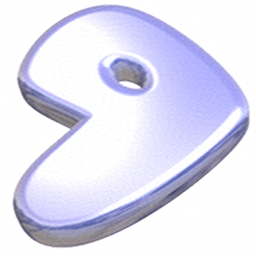
\includegraphics[width=\textwidth]{plaatjes/gentoo_fourier_0_15.png}
  \end{subfigure}
  \begin{subfigure}[b]{0.24\textwidth}
    \centering
    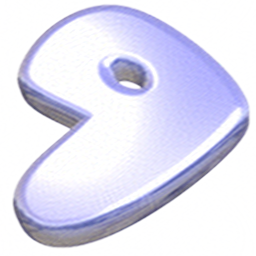
\includegraphics[width=\textwidth]{plaatjes/gentoo_fourier_0_1.png}
  \end{subfigure}
  \begin{subfigure}[b]{0.24\textwidth}
    \centering
    
\includegraphics[width=\textwidth]{plaatjes/gentoo_fourier_0_05.png}
  \end{subfigure}
  \begin{subfigure}[b]{0.24\textwidth}
    \centering
    
\includegraphics[width=\textwidth]{plaatjes/gentoo_fourier_0_01.png}
  \end{subfigure}
  \caption{Fourier op compressieniveaus 0.15, 0.10, 0.05, 0.01.}
\end{figure}
\begin{figure}
  \centering
  \begin{subfigure}[b]{0.24\textwidth}
    \centering
    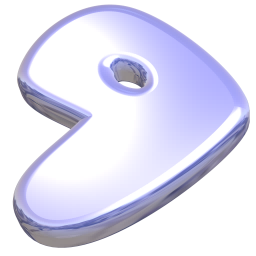
\includegraphics[width=\textwidth]{plaatjes/gentoo_haar_0_15.png}
  \end{subfigure}
  \begin{subfigure}[b]{0.24\textwidth}
    \centering
    
\includegraphics[width=\textwidth]{plaatjes/gentoo_haar_0_1.png}
  \end{subfigure}
  \begin{subfigure}[b]{0.24\textwidth}
    \centering
    
\includegraphics[width=\textwidth]{plaatjes/gentoo_haar_0_05.png}
  \end{subfigure}
  \begin{subfigure}[b]{0.24\textwidth}
    \centering
    
\includegraphics[width=\textwidth]{plaatjes/gentoo_haar_0_01.png}
  \end{subfigure}
  \caption{Haar op compressieniveaus 0.15, 0.10, 0.05, 0.01.}
\end{figure}
\begin{figure}
  \centering
  \begin{subfigure}[b]{0.24\textwidth}
    \centering
    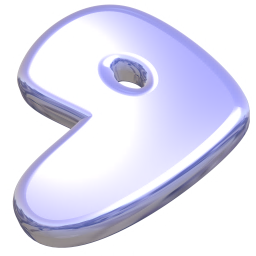
\includegraphics[width=\textwidth]{plaatjes/gentoo_db2_0_15.png}
  \end{subfigure}
  \begin{subfigure}[b]{0.24\textwidth}
    \centering
    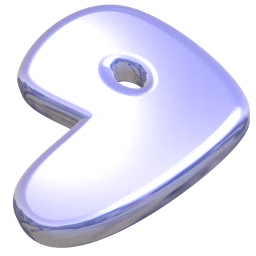
\includegraphics[width=\textwidth]{plaatjes/gentoo_db2_0_1.png}
  \end{subfigure}
  \begin{subfigure}[b]{0.24\textwidth}
    \centering
    
\includegraphics[width=\textwidth]{plaatjes/gentoo_db2_0_05.png}
  \end{subfigure}
  \begin{subfigure}[b]{0.24\textwidth}
    \centering
    
\includegraphics[width=\textwidth]{plaatjes/gentoo_db2_0_01.png}
  \end{subfigure}
  \caption{Daubechies 2 op compressieniveaus 0.15, 0.10, 0.05, 0.01.}
\end{figure}
\begin{figure}
  \centering
  \begin{subfigure}[t]{0.48\textwidth}
    \centering
    \vspace{10pt}
    \begingroup

    \renewcommand*{\arraystretch}{1.5}
    $\begin{array}{c | c c c c}
      \text{Compr} & \text{Fourier} & \text{Haar} & \text{DB2} \\ \hline
      0.150 & -21.564987 & 1.508043 & -0.325757 \\
      0.125 & -22.220604 & -3.607729 & -4.753701 \\
      0.100 & -22.974077 & -7.518578 & -8.964313 \\
      0.075 & -23.893526 & -11.909545 & -13.080699 \\
      0.050 & -25.134504 & -17.028756 & -17.498265 \\
      0.040 & -25.786567 & -19.471026 & -19.515331 \\
      0.030 & -26.597406 & -21.936183 & -21.791275 \\
      0.020 & -27.693270 & -25.283096 & -24.377904 \\
      0.010 & -29.532364 & -28.763393 & -27.638580 \\ \hline
    \end{array}$
    \endgroup
  \end{subfigure}
  \begin{subfigure}[t]{0.48\textwidth}
    \centering
    \vspace{0pt}
    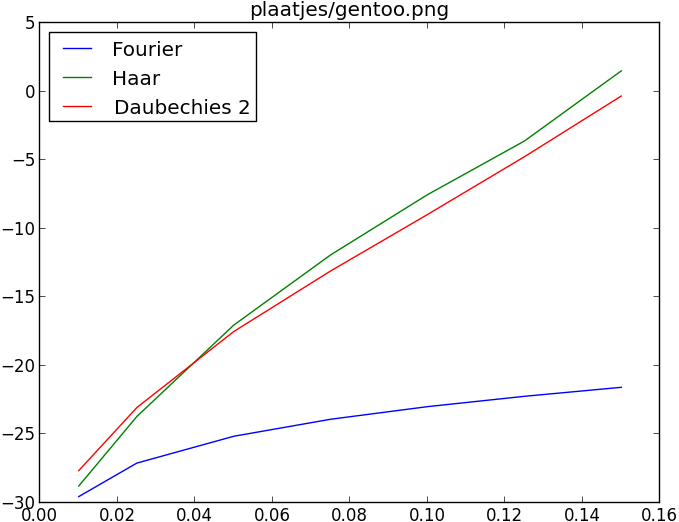
\includegraphics[height=\textwidth]{plaatjes/grafiek_gentoo_0_15-0_01.png}
  \end{subfigure}
  \caption{Grafiek en PSNR.}
\end{figure}
\restoregeometry
\pagebreak


\pagebreak
\newgeometry{left=2cm,right=2cm,top=1cm,bottom=1cm}
\begin{figure}
  \centering
  \begin{subfigure}[b]{0.24\textwidth}
    \centering
    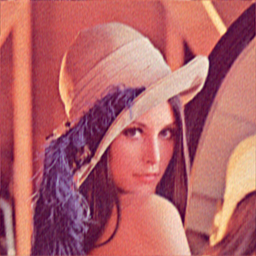
\includegraphics[width=\textwidth]{plaatjes/Lenna_fourier_0_1.png}
  \end{subfigure}
  \begin{subfigure}[b]{0.24\textwidth}
    \centering
    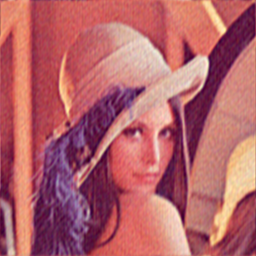
\includegraphics[width=\textwidth]{plaatjes/Lenna_fourier_0_05.png}
  \end{subfigure}
  \begin{subfigure}[b]{0.24\textwidth}
    \centering
    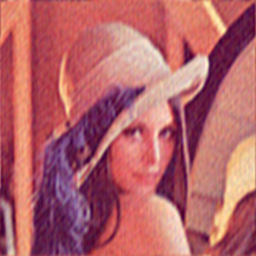
\includegraphics[width=\textwidth]{plaatjes/Lenna_fourier_0_03.png}
  \end{subfigure}
  \begin{subfigure}[b]{0.24\textwidth}
    \centering
    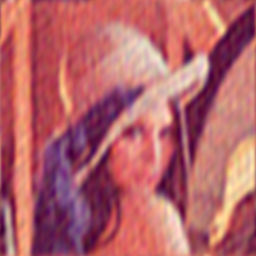
\includegraphics[width=\textwidth]{plaatjes/Lenna_fourier_0_01.png}
  \end{subfigure}
  \caption{Fourier op compressieniveaus 0.10, 0.05, 0.03, 0.01.}
\end{figure}
\begin{figure}
  \centering
  \begin{subfigure}[b]{0.24\textwidth}
    \centering
    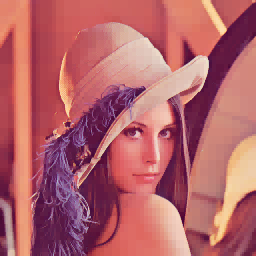
\includegraphics[width=\textwidth]{plaatjes/Lenna_haar_0_1.png}
  \end{subfigure}
  \begin{subfigure}[b]{0.24\textwidth}
    \centering
    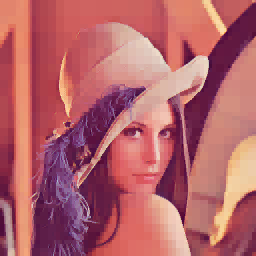
\includegraphics[width=\textwidth]{plaatjes/Lenna_haar_0_05.png}
  \end{subfigure}
  \begin{subfigure}[b]{0.24\textwidth}
    \centering
    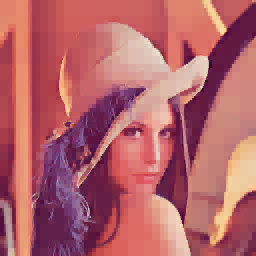
\includegraphics[width=\textwidth]{plaatjes/Lenna_haar_0_03.png}
  \end{subfigure}
  \begin{subfigure}[b]{0.24\textwidth}
    \centering
    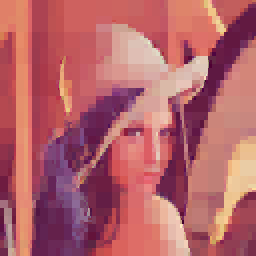
\includegraphics[width=\textwidth]{plaatjes/Lenna_haar_0_01.png}
  \end{subfigure}
  \caption{Haar op compressieniveaus 0.10, 0.05, 0.03, 0.01.}
\end{figure}
\begin{figure}
  \centering
  \begin{subfigure}[b]{0.24\textwidth}
    \centering
    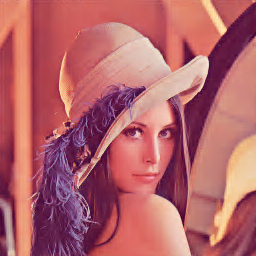
\includegraphics[width=\textwidth]{plaatjes/Lenna_db2_0_1.png}
  \end{subfigure}
  \begin{subfigure}[b]{0.24\textwidth}
    \centering
    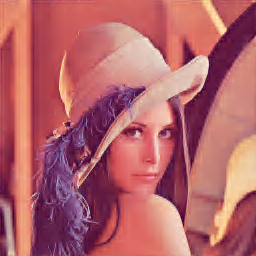
\includegraphics[width=\textwidth]{plaatjes/Lenna_db2_0_05.png}
  \end{subfigure}
  \begin{subfigure}[b]{0.24\textwidth}
    \centering
    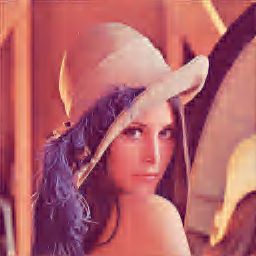
\includegraphics[width=\textwidth]{plaatjes/Lenna_db2_0_03.png}
  \end{subfigure}
  \begin{subfigure}[b]{0.24\textwidth}
    \centering
    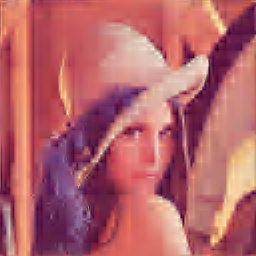
\includegraphics[width=\textwidth]{plaatjes/Lenna_db2_0_01.png}
  \end{subfigure}
  \caption{Daubechies 2 op compressieniveaus 0.10, 0.05, 0.05, 0.01.}
\end{figure}
\begin{figure}
  \centering
  \begin{subfigure}[t]{0.48\textwidth}
    \centering
    \vspace{10pt}
    \begingroup

    \renewcommand*{\arraystretch}{1.5}
    $\begin{array}{c | c c c c}
      \text{Compr} & \text{Fourier} & \text{Haar} & \text{DB2} \\ \hline
      0.200 & -21.043701 & -16.443978 & -15.615197 \\
      0.100 & -23.867860 & -20.863769 & -20.134351 \\
      0.050 & -25.825943 & -24.400495 & -23.745103 \\
      0.040 & -26.362758 & -25.303459 & -24.684358 \\
      0.030 & -27.024421 & -26.407813 & -25.757180 \\
      0.020 & -27.928360 & -27.754692 & -27.139561 \\
      0.010 & -29.380617 & -29.651147 & -29.111878 \\ \hline
    \end{array}$
    \endgroup
  \end{subfigure}
  \begin{subfigure}[t]{0.48\textwidth}
    \centering
    \vspace{0pt}
    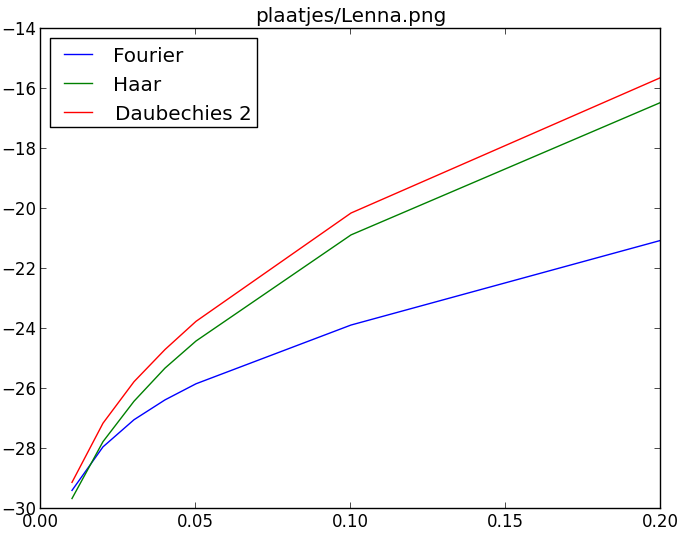
\includegraphics[height=\textwidth]{plaatjes/grafiek_Lenna_0_15-0_01.png}
  \end{subfigure}
  \caption{Grafiek en PSNR.}
\end{figure}
\restoregeometry
\pagebreak

\pagebreak
\newgeometry{left=2cm,right=2cm,top=1cm,bottom=1cm}
\begin{figure}
  \centering
  \begin{subfigure}[b]{0.24\textwidth}
    \centering
    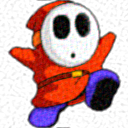
\includegraphics[width=\textwidth]{plaatjes/shyguy_fourier_0_1.png}
  \end{subfigure}
  \begin{subfigure}[b]{0.24\textwidth}
    \centering
    
\includegraphics[width=\textwidth]{plaatjes/shyguy_fourier_0_05.png}
  \end{subfigure}
  \begin{subfigure}[b]{0.24\textwidth}
    \centering
    
\includegraphics[width=\textwidth]{plaatjes/shyguy_fourier_0_03.png}
  \end{subfigure}
  \begin{subfigure}[b]{0.24\textwidth}
    \centering
    
\includegraphics[width=\textwidth]{plaatjes/shyguy_fourier_0_01.png}
  \end{subfigure}
  \caption{Fourier op compressieniveaus 0.10, 0.05, 0.03, 0.01.}
\end{figure}
\begin{figure}
  \centering
  \begin{subfigure}[b]{0.24\textwidth}
    \centering
    
\includegraphics[width=\textwidth]{plaatjes/shyguy_haar_0_1.png}
  \end{subfigure}
  \begin{subfigure}[b]{0.24\textwidth}
    \centering
    
\includegraphics[width=\textwidth]{plaatjes/shyguy_haar_0_05.png}
  \end{subfigure}
  \begin{subfigure}[b]{0.24\textwidth}
    \centering
    
\includegraphics[width=\textwidth]{plaatjes/shyguy_haar_0_03.png}
  \end{subfigure}
  \begin{subfigure}[b]{0.24\textwidth}
    \centering
    
\includegraphics[width=\textwidth]{plaatjes/shyguy_haar_0_01.png}
  \end{subfigure}
  \caption{Haar op compressieniveaus 0.10, 0.05, 0.03, 0.01.}
\end{figure}
\begin{figure}
  \centering
  \begin{subfigure}[b]{0.24\textwidth}
    \centering
    
\includegraphics[width=\textwidth]{plaatjes/shyguy_db2_0_1.png}
  \end{subfigure}
  \begin{subfigure}[b]{0.24\textwidth}
    \centering
    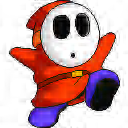
\includegraphics[width=\textwidth]{plaatjes/shyguy_db2_0_05.png}
  \end{subfigure}
  \begin{subfigure}[b]{0.24\textwidth}
    \centering
    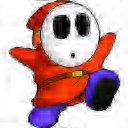
\includegraphics[width=\textwidth]{plaatjes/shyguy_db2_0_03.png}
  \end{subfigure}
  \begin{subfigure}[b]{0.24\textwidth}
    \centering
    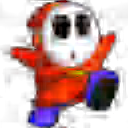
\includegraphics[width=\textwidth]{plaatjes/shyguy_db2_0_01.png}
  \end{subfigure}
  \caption{Daubechies 2 op compressieniveaus 0.10, 0.05, 0.05, 0.01.}
\end{figure}
\begin{figure}
  \centering
  \begin{subfigure}[t]{0.48\textwidth}
    \centering
    \vspace{10pt}
    \begingroup

    \renewcommand*{\arraystretch}{1.5}
    $\begin{array}{c | c c c c}
      \text{Compr} & \text{Fourier} & \text{Haar} & \text{DB2} \\ \hline
      0.125 & -25.709419 & 6.188436 & -12.939796 \\
      0.100 & -26.352690 & -2.252695 & -16.684428 \\
      0.075 & -27.084570 & -13.247047 & -20.121718 \\
      0.050 & -27.987835 & -22.194021 & -23.640705 \\
      0.040 & -28.455719 & -25.861219 & -25.259163 \\
      0.030 & -29.045916 & -26.633403 & -26.750137 \\
      0.020 & -29.857696 & -28.858775 & -28.445793 \\
      0.010 & -31.289113 & -31.320495 & -30.669577 \\ \hline
    \end{array}$
    \endgroup
  \end{subfigure}
  \begin{subfigure}[t]{0.48\textwidth}
    \centering
    \vspace{0pt}
    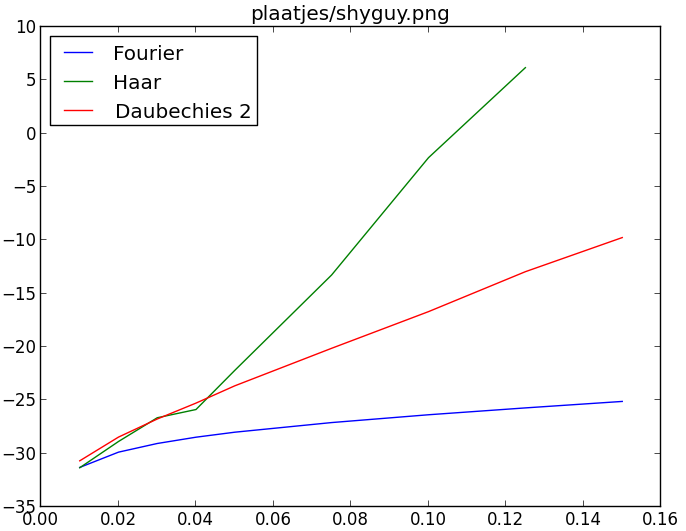
\includegraphics[height=\textwidth]{plaatjes/grafiek_shyguy_0_15-0_01.png}
  \end{subfigure}
  \caption{Grafiek en PSNR.}
\end{figure}
\restoregeometry
\pagebreak

\chapter{Reflectie en discussie}
In dit laatste hoofdstuk zullen we een meta-analyse maken van de praktische resultaten. Bladiebla TODO.

Wanneer we kijken naar de grafieken, wordt het direct duidelijk dat de Fouriertransformatie in eigenlijk alle gevallen een slechter resultaat oplevert (zowel in `wolligheid' als gereflecteerd door de PSNR).
\chapter{Populaire samenvatting}

\begin{thebibliography}{11}
\addcontentsline{toc}{chapter}{Bibliografie} 

\bibitem{akra-bazzi}
  Mohamad Akra, Louay Bazzi,
  \emph{On the solution of linear recurrence equations}.
  Computational Optimization and Applications,
  10(2):195 - 210,
  1998.

\bibitem{fourier-fout}
  Bochner S., Chandrasekharan K.
  \emph{Fourier Transforms}.
  Princeton University Press.
  1949.

\bibitem{wavelet_filter}
  \url{http://djj.ee.ntu.edu.tw/Wavelet_Filter.pdf}

\bibitem{tammo}
  Tammo Jan Dijkstra,
  \emph{Adaptive tensor product wavelet methods for solving PDEs}, 2009
\bibitem{tensor_wavelet}
  \url{http://www.uio.no/studier/emner/matnat/math/MAT-INF2360/v12/tensorwavelet.pdf}
\bibitem{mallat}
  St\'ephane Mallat,
  \emph{A Wavelet Tour of Signal Processing}
\bibitem{jackson}
  \url{http://www.ams.org/journals/bull/1960-66-02/S0002-9904-1960-10426-0/S0002-9904-1960-10426-0.pdf}

\bibitem{daubechies}
  Ingrid Daubechies, \emph{Orthonormal Bases of Compactly Supported Wavelets}.
  AT\&T Bell Laboratories, 1988.
\bibitem{parseval}
  \url{http://www.encyclopediaofmath.org/index.php/Parseval_equality}

\end{thebibliography}

\end{document}
